\documentclass[a4paper,12pt]{article}
\usepackage[utf8]{inputenc}
\usepackage{fancyhdr}
\usepackage{enumerate}
\usepackage{graphicx}
\usepackage{float}
\restylefloat{table}
\pagestyle{fancy}
\usepackage{url}
\fancyhfoffset[LE]{6mm}
\usepackage{listings}
\usepackage{color}
\usepackage{subfig}
\usepackage{setspace}
\usepackage[margin=1 in]{geometry}
\usepackage[toc,page]{appendix}

\definecolor{dkgreen}{rgb}{0,0.6,0}
\definecolor{gray}{rgb}{0.5,0.5,0.5}
\definecolor{mauve}{rgb}{0.58,0,0.82}

\lstset{frame=tb,
  language=C,
  aboveskip=3mm,
  belowskip=3mm,
  showstringspaces=false,
  columns=flexible,
  basicstyle={\small\ttfamily},
  numbers=left, 
  numberstyle=\tiny\color{gray},
  keywordstyle=\color{blue},
  commentstyle=\color{dkgreen},
  stringstyle=\color{mauve},
  breaklines=true,
  breakatwhitespace=true,
  tabsize=3
}

\lhead{Li, Yang, Zhang}
\rhead{COMP3203 Final Project Report - Page \thepage}
\cfoot{Carleton University - December 17, 2015}
\renewcommand{\headrulewidth}{0.4pt}
\renewcommand{\footrulewidth}{0.4pt}
\setlength{\parindent}{4ex}

\title{BlueStream \\ Final Project Report}
\author{Li, Charlie (100832579) \\ Yang, Yinuo () \\ Zhang, Hector (100947935) }
\date{December 17, 2015}
\begin{document}
\maketitle

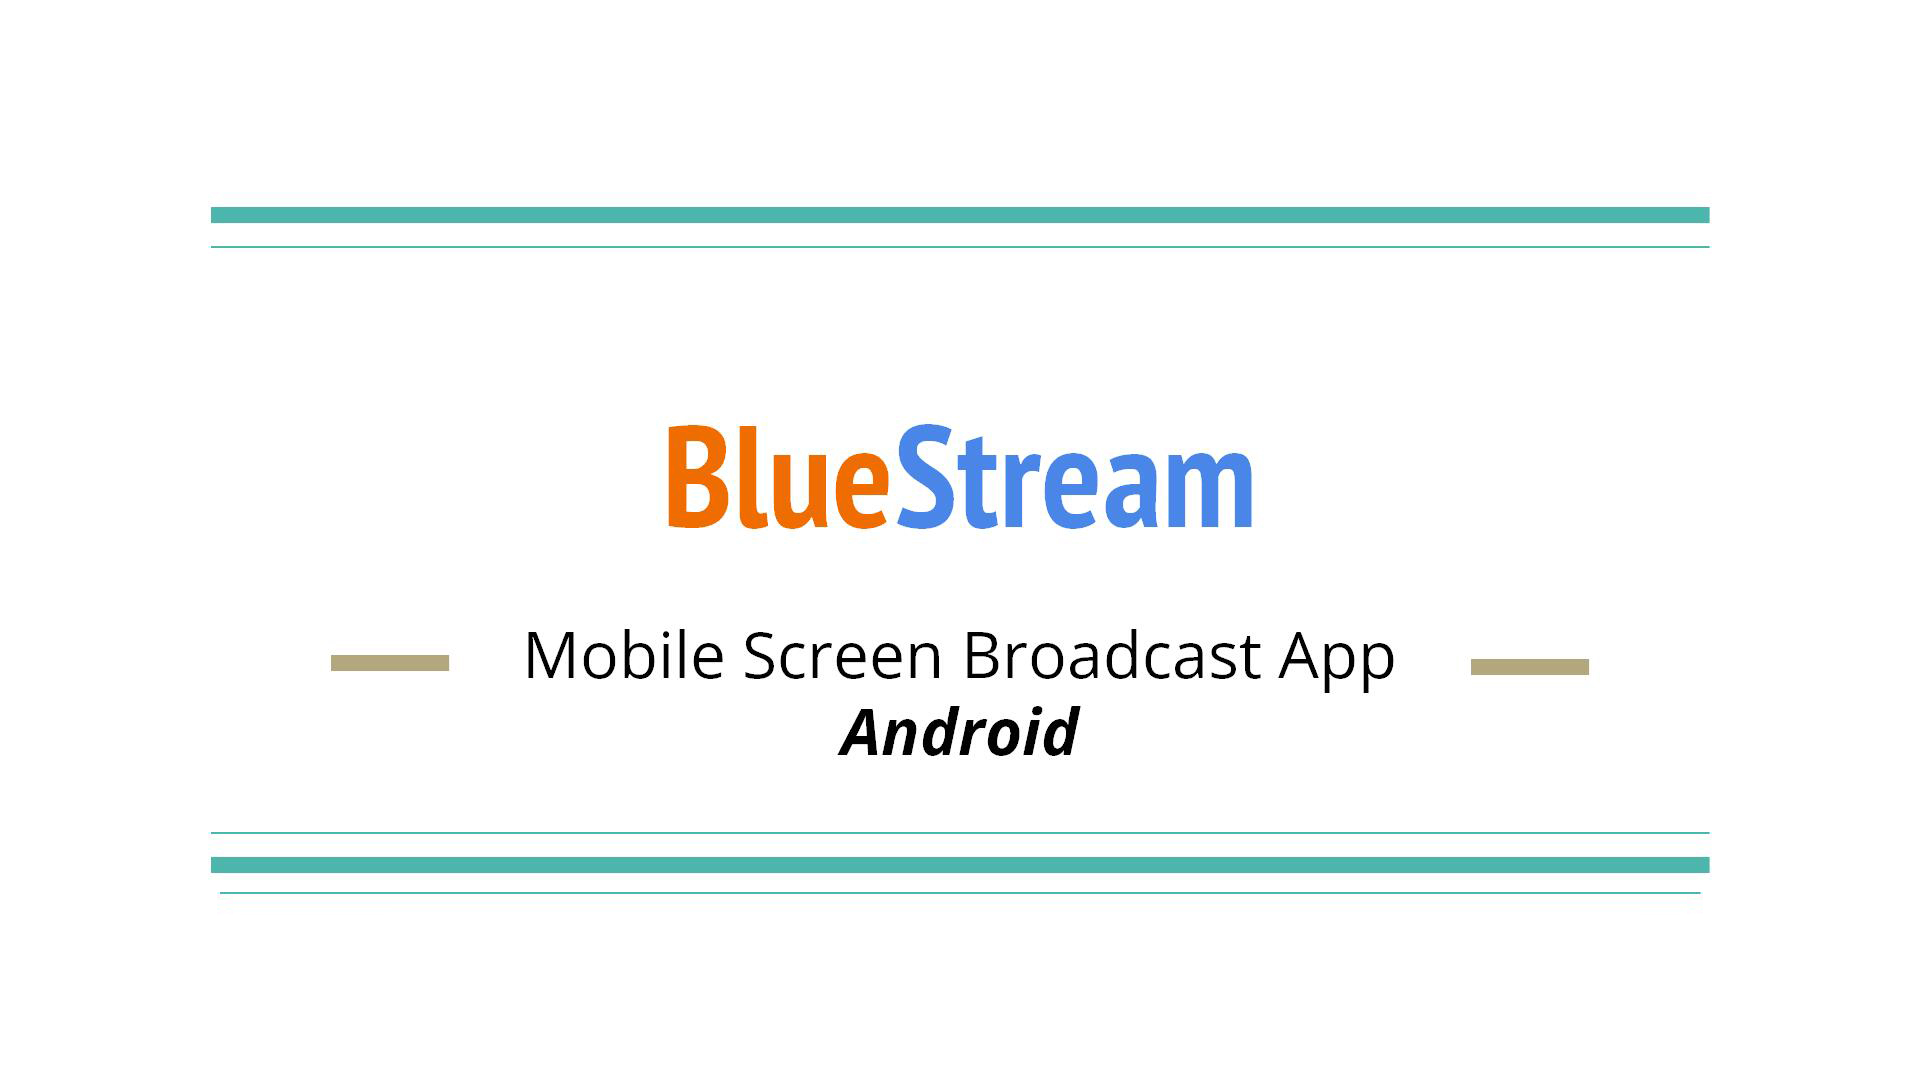
\includegraphics[scale=.2]{BlueStream.jpg}
\newpage
\tableofcontents
\newpage
\section{Introduction}


\subsection{Context}
BlueStream is a mobile screen broadcasting android application that communicates through Bluetooth (BT) wireless technology. This section provides some light details on the technology used for our mobile application, the device runtime environment, and some background concepts needed to proceed to further sections. The main functionality that BlueStream provides to the end user is the ability to share the current state of mobile display to another user in close proximity over wireless connection. BT is a short range wireless technology standard for exchanging data over short distances, in our case, from mobile device to device over radio waves. The form of data transfer that BT uses is short-wavelength, ultra high frequence (UHF) radio waves which are a category of electromagnetic radiation with lower signal frequency and vary in wavelengths that are longer than infrared and microwave. UHF is designated by the international telecommunication union to operate in frequency ranges of 300 MHz to 3 GHz. Frequencies in this range are also known as the decimetre band, where the range of the wave signal is between one meter to ten meters. Within this decimetre band, resides the infamous 2.4GHz to 2.485GHz band that were reserved for industrial, scientific, and medical (ISM) radio bands established in 1985 and is globally unlicensed. BT was designed to work out the shortcomings of its higher frequency, shorter wavelength sibling, the infrared light, by enabling a faster transfer speed, and eliminating the need for light of sight communication.

In the beginning of a connection, BlueStream uses a BT Service Discovery Protocol (SDP) to discover and connect to nearby users within 10 meter range (class 2 BT). Once connected, BlueStream uses a packet transmission protocol named Radio Frequency Communication (RFCOMM). A detailed outlined in section two, the background, will depict the BR/EDR stack used to develop BlueStream. This protocol stack serves to define the set of transport protocols for managing two devices with a connected state is present. During the connection, BlueStream utilizes a frame compression format called Motion JPEG (M-JPEG) to transmit frames across the connection. Furthermore, this compression format is a part of the core streaming protocol that is developed for BlueStream. Our runtime environment that is used to test BlueStream is on mobile smart phone platforms that run Lollipop 5.0 or greater on the Linux kernel 3.4. The test devices all are quad core running between 2.3-2.5 GHz and loaded with 2 gigabytes of random access memory running the Adreno 330 graphics processor. Figure \ref{fig:DeviceProfiles} shows the specifications of our test device to contrast the slower device A, and faster device B. Over the scope of this report, these devices, by their IDs (A or B) will be referenced regularly. This wraps up all necessary contextual information about the BlueStream application and now, let's provide a description of the problem the development team had to face during the application development process.

\begin{figure}[h!]
\centering
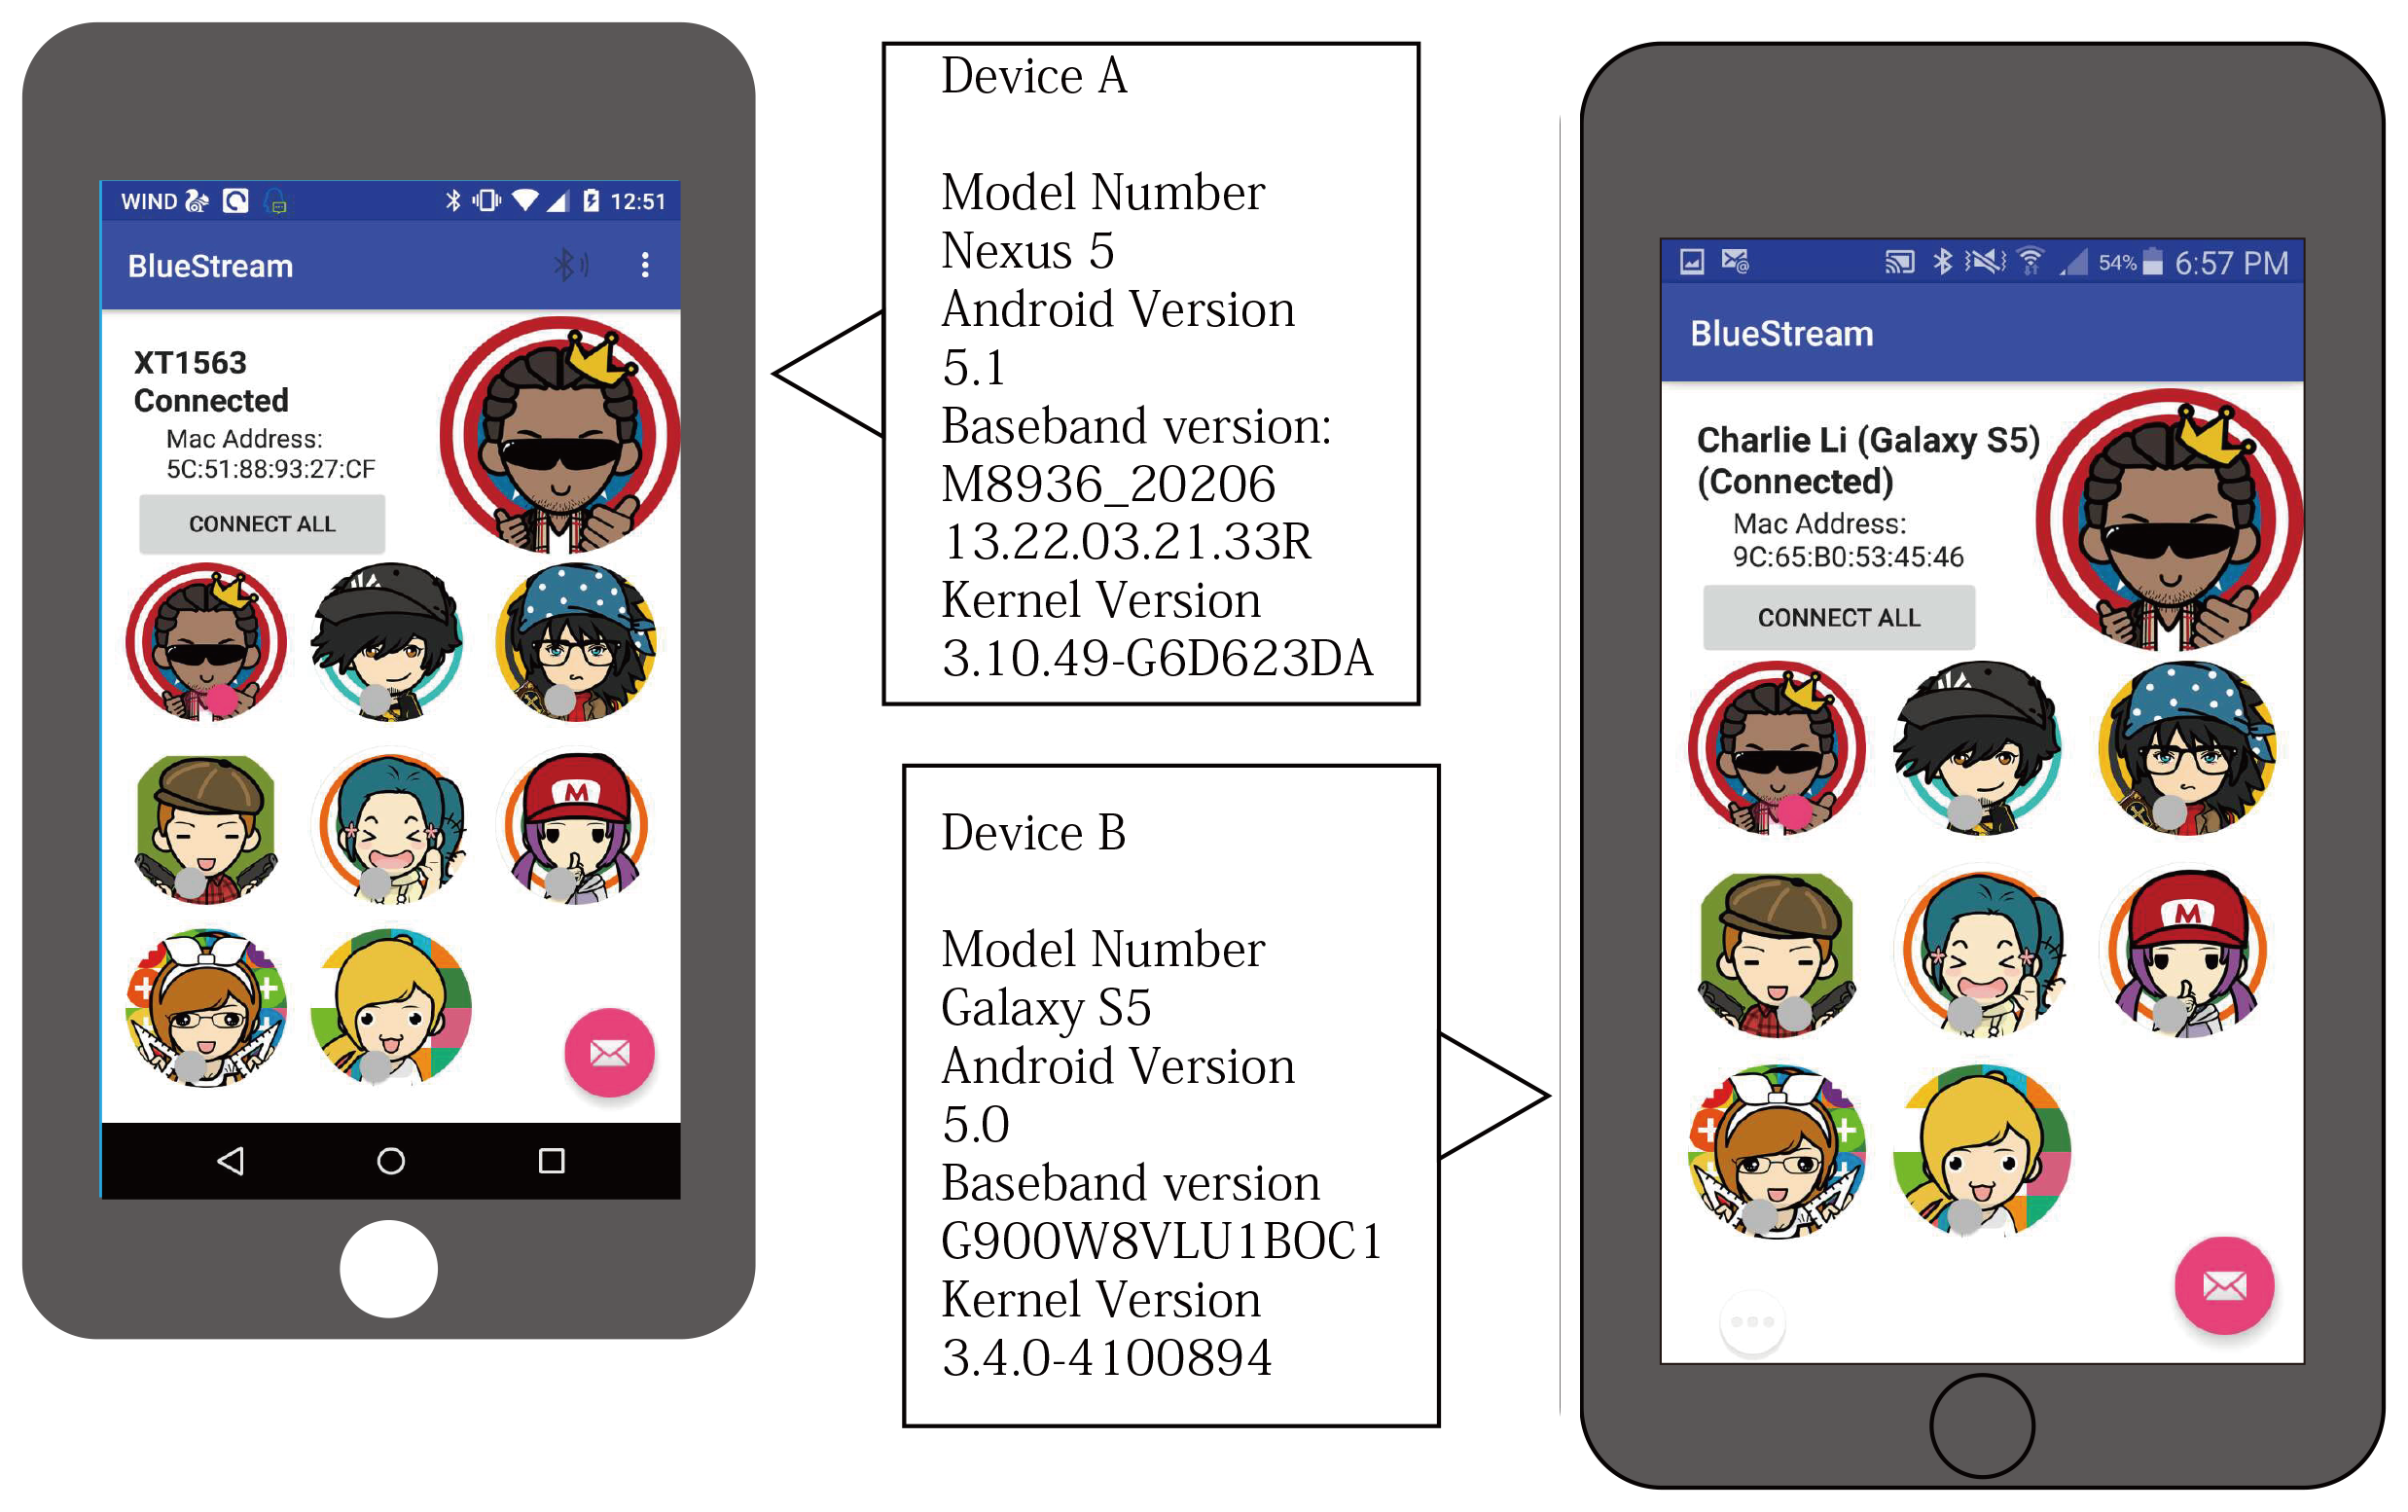
\includegraphics[scale=.6]{Figures/Figure1.png}
\caption{Profiles of Device A and Device B}
\label{fig:DeviceProfiles}
\end{figure}

\subsection{Problem Statement}
Our main background motivation for BlueStream came from the popular game streaming service Twitch. Instead of targeting major viewers on the internet, we wanted to build a peer to peer streaming service the user can use on their smartphones anywhere. BlueStream approaches the problem of inter-device communication by capturing the screen of a smartphone and streaming the contents to another phone. As the devices described in Figure \ref{fig:DeviceProfiles} show the two smartphones participating in this activity. Device A will capture the movements in its screen and streams the contents to device B, who is currently maintaining a connection to view the screen of device A. The roles can also be reversed where device A views device B’s screen. The main design goal for BlueStream was to optimize the performance of the stream while maintaining usability of the application. This problem is relevant to the communication medium in which we have chosen Bluetooth (BT) because technology constraints on the data rate. Stream quality becomes an important issue as higher higher quality video streams require higher bandwidth and then optimizing these traits becomes a balance of quality and performance to find an intersection for the best usability experience. Over the course of this report, we will be identifying and analyzing the video stream algorithm for bottlenecks and external environment factors and conclude with an explanation of why we think the settings we choose, best fits our goal. 

\subsection{Result}
The fruits of our labour yielded us an working, optimized screen sharing application, capable to stream and view the screen to and from another smartphone through the Bluetooth wireless technology. We solved our problem, described in section 1.2, by utilizing a frame compression format call M-JPEG in our streaming algorithm that allowed us to fine tune our streaming service to provide the best quality in respect to the usability of our application. Our algorithm highlights the capture of single frames from the streaming device’s desktop operating system in real time and the ability to condense each frame to an optimal size to be transfer over the BT wireless connection. BlueStream highlights a peer to peer architecture to allow this stream work in both directions of connected peers. 

In order to determine the most optimal degree of performance, we have analyzed our algorithm through performance benchmarking (using frames per second as the performance metric) and usability surveying. During performance benchmarks, our tests targets parts of the algorithm and external environment to identify factors that will degrade the performance of the application. The factors include the processing time of a single frame (capture + compression + serialization), quality of the frame in respect to the size of the payload transfer time, the distance between two devices, and runtime environments where there exists high and low noise (signals within the ISM band). 


\subsection{Outline}
\textbf{Section 2: Background} is aimed to present the necessary information need to justify the result and evaluation of the project. This section will focus on bringing the reader up to speed with the BT technology standards and M-JPEG that are implemented for BlueStream. This section will make contracts towards the OSI model where each layer is described in detailed about its significance and role in the BlueStream application. \\

\noindent\textbf{Section 3: Result} is to provide the reader with solid proof and performance benchmarks made for the final project result. This section includes the UML Diagram and architecture of BlueStream, the algorithm of the core frame transferring mechanism, and graphs relating to the complexity models of the project. Additionally, this section will contract the effect of different interferences during streaming such as determining the extent of signal strength, distance, processing time and image size could have on the performance of the application.\\

\noindent\textbf{Section 4: Evaluation} is devoted to assess the performance of the application, referencing graphic depictions of data captured in Section 3: Result to critically evaluate the current state of BlueStream. Due to the time constraints of this project, this section will generate reasoning behind the perceived results in context to how the technologies used for BlueStream,impacted those results and how they could be improved. Lastly, this section will address the extend to how the goals had been met over the development of the BlueStream application.  \\

\noindent\textbf{Section 5: Conclusion} will summarize and highlight the main achievements BlueStream had reached, any future works, and the contribution of each team members followed by a bibliography referencing all the resources that aiding the development of the application.



\section{Background}
The BlueStream mobile application is intended to be developed to solve the issue of remote screen sharing across a short distance. Sometimes a user may find it easier to show what is happening on their device rather than explaining it through long message transactions. Screen sharing has been a popular way to show another person how to use a smartphone to another user. From a practical perspective, screen sharing can aid in remote debugging, sharing entertainment, and sharing live video footage of one’s surroundings. 

Care has been taken to select and assess the appropriate wireless technology for this application. The technologies we considered for BlueStream was WiFi, cellular data services, satellite communications, and BT. The development team decided to rule out satellite communications due to infeasibility in its costs and latency in performance and directed our attention to towards the latter. Sharing videos and streaming is a resource greedy activity that all mobile users must tolerate. In Canada, mobile plans for unlimited data transfer can cost upwards of a hundred dollars per month. Coverage for 3G, 4G, also do not span across country lands and is very limited in suburban locations throughout the country. We found cellular data services to be expensive and is also limited by the coverage, and hence the possibility had been opted out. WiFi is a promising medium for communications however, it’s heavily reliant on a local router than can process application packets to the internet and put constraints on where BlueStream could be used from. In that case, making a mobile application became obsolete since the factor of mobility become a function of how close the user was to a router access point.

BlueStream approaches the problems by eliminating the data transfer cap and allow all devices to connect in any circumstance as long as they are within the BT designated range, independent of a central router and at zero cost on the wallet. The goal for this application is to provide the user with mobile screen sharing utility that can function in any part of the world, under any circumstances within the boundaries of the technology, and cost virtually nothing to transfer a stream for as long as the batteries on each device will allow. Security is also one of the primary problems that BlueStream addresses when using the low footprint BT technology. BT packets do not route through a central server and thus, anonymity is preserved. 

Nowadays, developing on the Android platform instantly associates the developer with a rich set of APIs that unlock the full power of sensors, image processing libraries, and wireless protocols in smart phones right off the bat. Some of these APIs include but are not limited to the Bluetooth 4.0 (BT) connection protocol library, which is used extensively in BlueStream for wireless communication. Over the years, the BT protocol has grown in maturity and is making the technology an easy to use full duplex (communication in both direction), low power consumption, and secure technology standard for short distance communication. The protocol level provides connected devices with a standard method of agreement to when bits are transmitted, how many will be transmitted at a time, and how the connected members can validate that the message received is the same as the message that was sent.

BT uses a technique called spread-spectrum frequency hopping when transferring information from one device to another. It’s just as the name suggests, the BT chip in a device will randomly choose 79 individual frequencies of 1MHZ within a designated range and apply such frequency changes 1,600 times a second, virtually eliminating collisions between other non connected devices \cite{InsideBlueTooth}. When two BT devices initiates a connection, a the BT protocol transaction takes place to determine if they have data to share or if one needs to control the other. Support for a maximum of 8 connection devices is made possible by the protocol where the devices create a personal-area network (PAN) or piconet. Once the devices are connected, they send messages to one another to synchronize the random frequency hops so they may transmit at the same frequency and avoid other BT devices that are running other random frequency hops. In terms of our application, BlueStream first synchronizes the spread-spectrum frequency hopping with its connecting party then transmits raw frames through the motion-JPEG (MJPEG) video compression format. 

This section will be broken down into two parts, providing in depth background into two of major parts of the BlueStream technology in order to provide its’ screen capture service. In order to make sense of this project’s result and further evaluate the behaviour of the application, it seems crucial to understand the actual wireless protocol driving the core technologies of this application. To start off, this section will explain the Bluetooth protocol stack and show how each layer is used the the communications between two mobile devices streaming video footage with BlueStream. After the low level components are explained, the last section will cover the application layer of BlueStream and depict its’ technologies and protocol used to stream video from one device to another.


\subsection{Bluetooth Protocol Stack}

Care has been taken to select the correct protocol that could fit the needs of BlueStream. The project was concerned with mainly two protocols as the last (high speed protocol) is not supported in android smart phones where writer John Pataki explained in a lovely article \cite{UnderstandingBTForAndroid}. 

\begin{enumerate}

\item Classic - the original protocol that supports BR/EDR (basic rate/enhanced data rate) and specifications are drawn from \cite{InsideBlueTooth}. 

\begin{enumerate}
\item supports 79 channels spaced by 1MHz 
\item connection time of roughly 20ms
\item supports scatternet, which can connect many piconets
\item has voice channels 
\item full duplex communication
\item 10 meter range
\item operates as both server (has data) and client (connection initiator) for app-to-app scenarios
\end{enumerate}
\item Low Energy - literally, the lighter protocol for BT communications that operates on a different model than classic mode:
    \begin{enumerate}
    \item supports 40 channels spaced by 1Mhz
    \item typically 30 to 100 meters range
    \item slower data rate
    \item does not support scatternets
    \item no voice channel
    \item must be the client that initiates the connection only
    \end{enumerate}
\end{enumerate}

As seen in the comparison above, BlueStream requires some fundamental services that BR/EDR provides such as a faster full duplex communication to maximize transfer time and dynamic service which enables the app to determine whether they can communicate as the server or client. The low energy protocol is more suitable to be used when paired with app-to-device (phone to peripheral) scenarios such as the app only need to initiate connections without having to listen for other smart phones. The Bluetooth BR/EDR protocol stack is defined as as series of layers similar to the Open Systems Interconnect (OSI) model of the web. Each layer in the stack is well partition to highlight the division of responsibility for communication. Each layer will be explained to the extent of practical use by the BlueStream app with the goal of optimizing the number of video frames are passed up and down the protocol stack. Figure \ref{fig:BTandOSIStack} depicts the BT stack in relation to the OSI Model, followed by a brief explanation of each layer where the specifications and details of the stack were provided by Jennifer Bray and Charles F. Sturman in reference \cite{ConnectWithoutCables}. In order to solidify the understanding of concepts and be unbiased to just one author the book Bluetooth Revealed by Brent Miller and Chatschik Bisdikian was studied to contract information between the books.

\begin{figure}[h!]
\centering
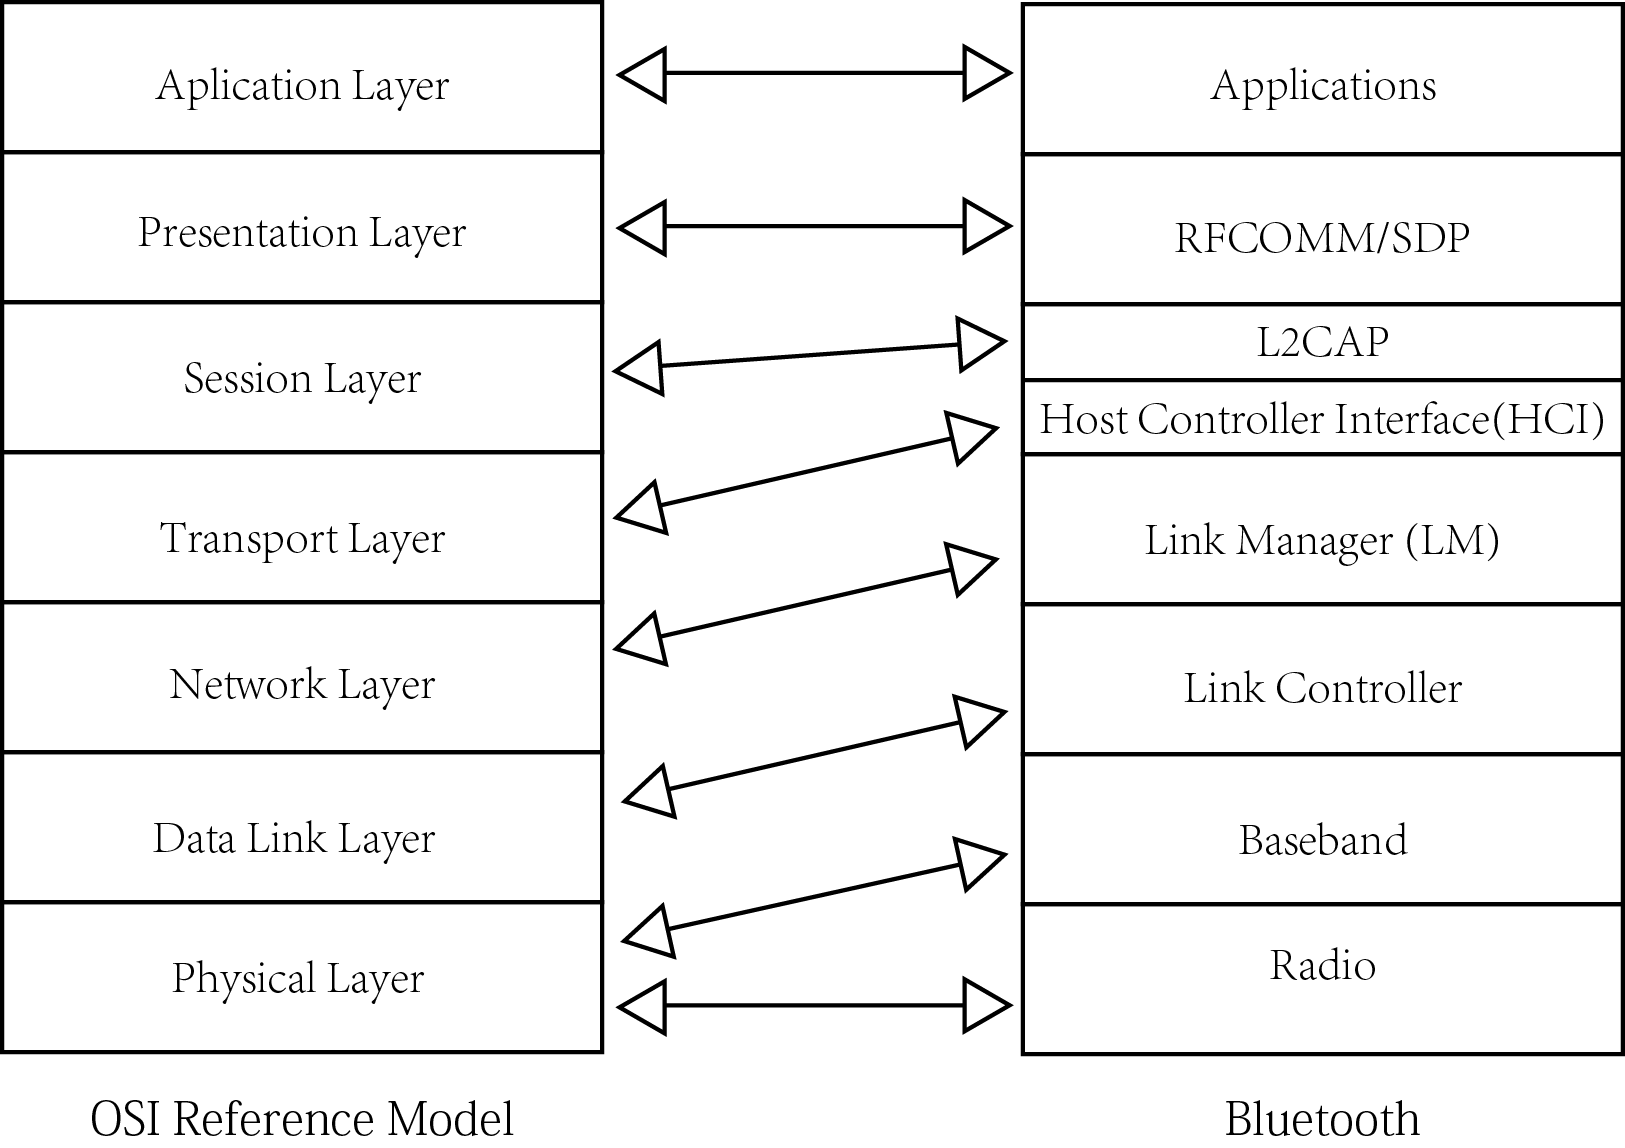
\includegraphics[scale=1]{Figures/Figure2.png}
\caption{The Bluetooth protocol stack in relation to the Open Systems Interconnect (OSI) model}
\label{fig:BTandOSIStack}
\end{figure}

\subsubsection{Radio Layer}
At the physical layer, the smartphones used to test BlueStream are embedded with a BT chip with an onboard antenna that transmits radio waves. An introduction of radio waves can refered to at section 1.1. The BT chips operate at 2.4GHz within the global ISM band, the same frequencies as WiFi. BlueStream’s chosen protocol BR/EDR uses 79 channels of this frequency range spaced into 1 MHz channels each radiating at 1 Megasymbol per second. According to Sturman, Bray, this is done to maximize the bandwidth of the channel. BT 4.0 uses a form of gaussian frequency shift keying modulation scheme that in theory can have a potential data rate of 24Mbps stated by Takuro Sato in Smart Grid Standard: Specification, Requirement, and Technologies \cite{SmartGrids}, however during testing, different data rates over the air were obtained and will be explained in the results section. 

As explained previously, 79 different channels are selected where to compose the spread-spectrum frequency hopping technique that allows the connection to retune to a different channel 1,600 times a second. Since one second is 1000 millisecond, BT only stays on one channel for 625 microseconds and the next is selected at pseudo random (there is an algorithm to determine the randomness)! Each time BT lands on a channel is called a slot. Generally a smart phone device will hop once per packet sent which can last either one slot, 3 slots, or 5 slots in time. This technique helps resolve a few important characteristics in the BT technology.

\begin{enumerate}
\item Noise interference on one channel may not be an impact when changing to another channel
\item Coalitions in one channel may occur, therefore sending a preceding packet in a different channel could minimize the retransfer to fail again
\end{enumerate}

The physical layer helps BT realize many potential safety nets to inter device communication through its frequency shifting technique. Next on top, the baseband layer will be explained.

\subsubsection{Baseband Layer}
The baseband layer is still considered a part of the physical layer in some Bluetooth technology textbooks, however there is a slight distinction between the two. The radio layer was concerned with the methods of transferring and receiving signal while the baseband is responsible for encoding, decoding, and low level timing management for the connection for each packet transfer. Each packet that BlueStream sends is in the form of a large image over the connection therefore the baseband layer must correctly time the transfer of the data packet over multiple slots and frequency hops. 

This layer initiates an asynchronous connection-less (ACL) link between the sending (server) and receiving (client) device. All user data must go through this link that acts a bus to the L2CAP layer (more on this later). Within a BT connection, there must be a leader host among the connection that becomes the master and all other a slave. The master is tasked to manage this connection and forward packets acting as a router (if the connection is a piconet). Over this link, the BT packet structure is also defined with having:

\begin{enumerate}
\item Access code section (68 bits) - identifies the packet as being from or to a specific master device. The section is comprised of mainly a synchronisation word and access codes used to help determine masters in a piconet.
\item Header section (54 bits) - this section contains control information associated to the packet. Some fields this header contains is active member address, packet type, and header error checker.
\item Payload section (0-2744 bits) - the actual data of the packet and is split into its own three parts:
    \begin{enumerate}
    \item Payload header - includes flow flags to control data transfer to the L2CAP layer, the length of the payload and the logical channel field to indicate whether is packet is the start or continuation of a L2CAP message. 
    \item Payload data - the good stuff
    \item Cyclic redundancy check (CRC) - used to make sure un corrupted data
    \end{enumerate}
\end{enumerate}

\begin{figure}[h!]
\centering
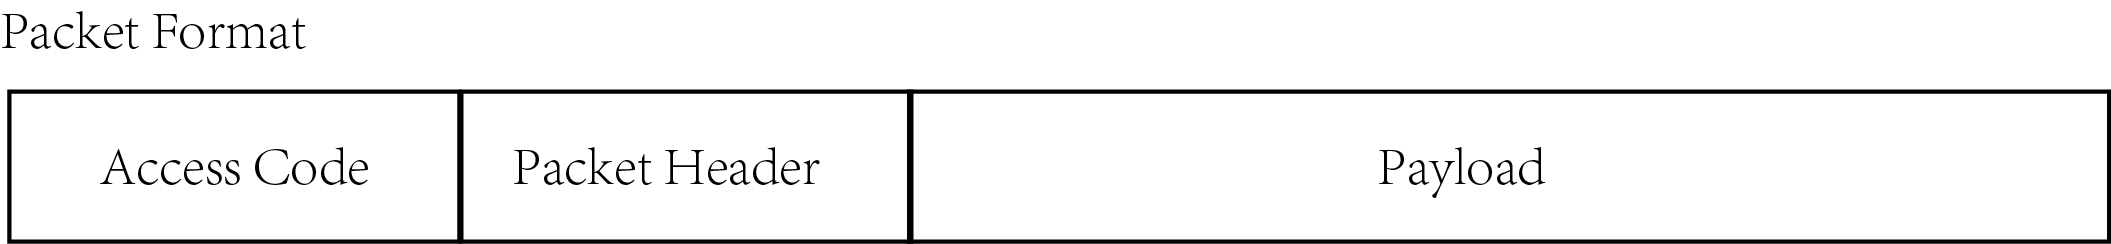
\includegraphics[scale=.8]{Figures/Figure3.png}
\caption{The Bluetooth Packet Format}
\label{fig:BTPacket}
\end{figure}

Figure \ref{fig:BTPacket} above shows the BT packet as described in this section. This contrasts the OSI model’s data link layer while baseband is partially physical as it controls packet timings in respect to frequency shifting as well as data link responsibilities such as encapsulating packets. The baseband layer ensures delivery of bytes in the same sequence it was segmented by the L2CAP layer using a form of sequence number number determined by the HCI layer to transfer the packets in the order that are meant to be sent. Up next, is the link controller layer.

\subsubsection{Link Controller Layer}
Right above baseband, there exists a link controller that provides controls to the link and packet-orientated connection. This layer has the responsibility to to maintain the link once the connection is set up. In case of error such as the times where the CRC does not check or packets are lost during the transmission, this layer utilizes the Acknowledgement/Request protocol to enable the retransmission of corrupted data. 

In BlueStream, the application’s link controller can maintain a few states:

\begin{enumerate}
\item Standby - the app is off
\item Inquiry and Inquiry Scan - when one instance of the app is trying to discover all BT enabled devices nearby using the Service Discovery Protocol (SDP). A request for essential information is sent to all nearby devices and when returned, this state builds up a table which includes the essential data to synchronize frequency hopping sequences and that forms a part of the access code section of the BT packet. 
\item Page and Page scan - determines a master from the connection. The master will then send paging messages containing information about the access code section of the BT packet to all the slaves in the piconet. 
\item Connection - a stable connected state with a few low power substates for hold, sniff, and park during periods where the devices are no busy. BlueStream is put in this state if two devices are not streaming, but will never enter low powered state during a stream. 
\end{enumerate}

There is a lot of details in this layer that is omitted for the purpose of brevity for this report. An essential part, the state transition diagram is not explain due to its’ complexity. However, in order to put the pieces together to form a rounded understanding of the BT stack, this section provided the basic information to understand how the technology in BlueStream works.

\subsubsection{Link Manager(LM) Layer}
BT stack has a great abstraction for the separation of concerns. In the layers previously described, the baseband layer provides a method of encapsulating data to be sent to the radio layer while the link controller manages the connection and determines who to send packets to. The link manager layer is another important aspect of this protocol that translates commands for  the Host Controller Interface (HCI) and can communicate to other link managers on other devices through a Link Management Protocol (LMP). Some operations and command this layer manages are:

\begin{enumerate}
\item Allocating member addresses for devices connecting to the BlueStream piconet
\item Ending connections between streaming devices
\item Configuring master and slave roles of a new connection or switching during connected state
\item Switch connections states to low power mode when BlueStream app is on standby
\item Establishing the ACL data link, used to communicate between the streaming and viewing device
\end{enumerate}

In summary, as the name suggests, this layer manages the connection and states of the running device and also communicating to other connected devices to inform them of decision that it made. Up next, the commands that this layer translated will go up to the HCI layer.

\subsubsection{Host Controller Interface(HCI) Layer}
This layer is used in conjunction to the Link Manager layer and drives the BlueStream service through the various of commands this layer receives from other layers such as baseband. The HCI serves as an application interface between the lower level and high level layers with the purpose of abstracting these two layers to integrate different implementations of the low and high level layer. This gives upper layers the flexibility to access baseband, link manager, and other hardware registers through this simplified interface as described by Brent Miller and Chatschik Bisdikian in the book \textit{Bluetooth Revealed}.

\begin{figure}[h!]
\centering
\hspace*{2cm}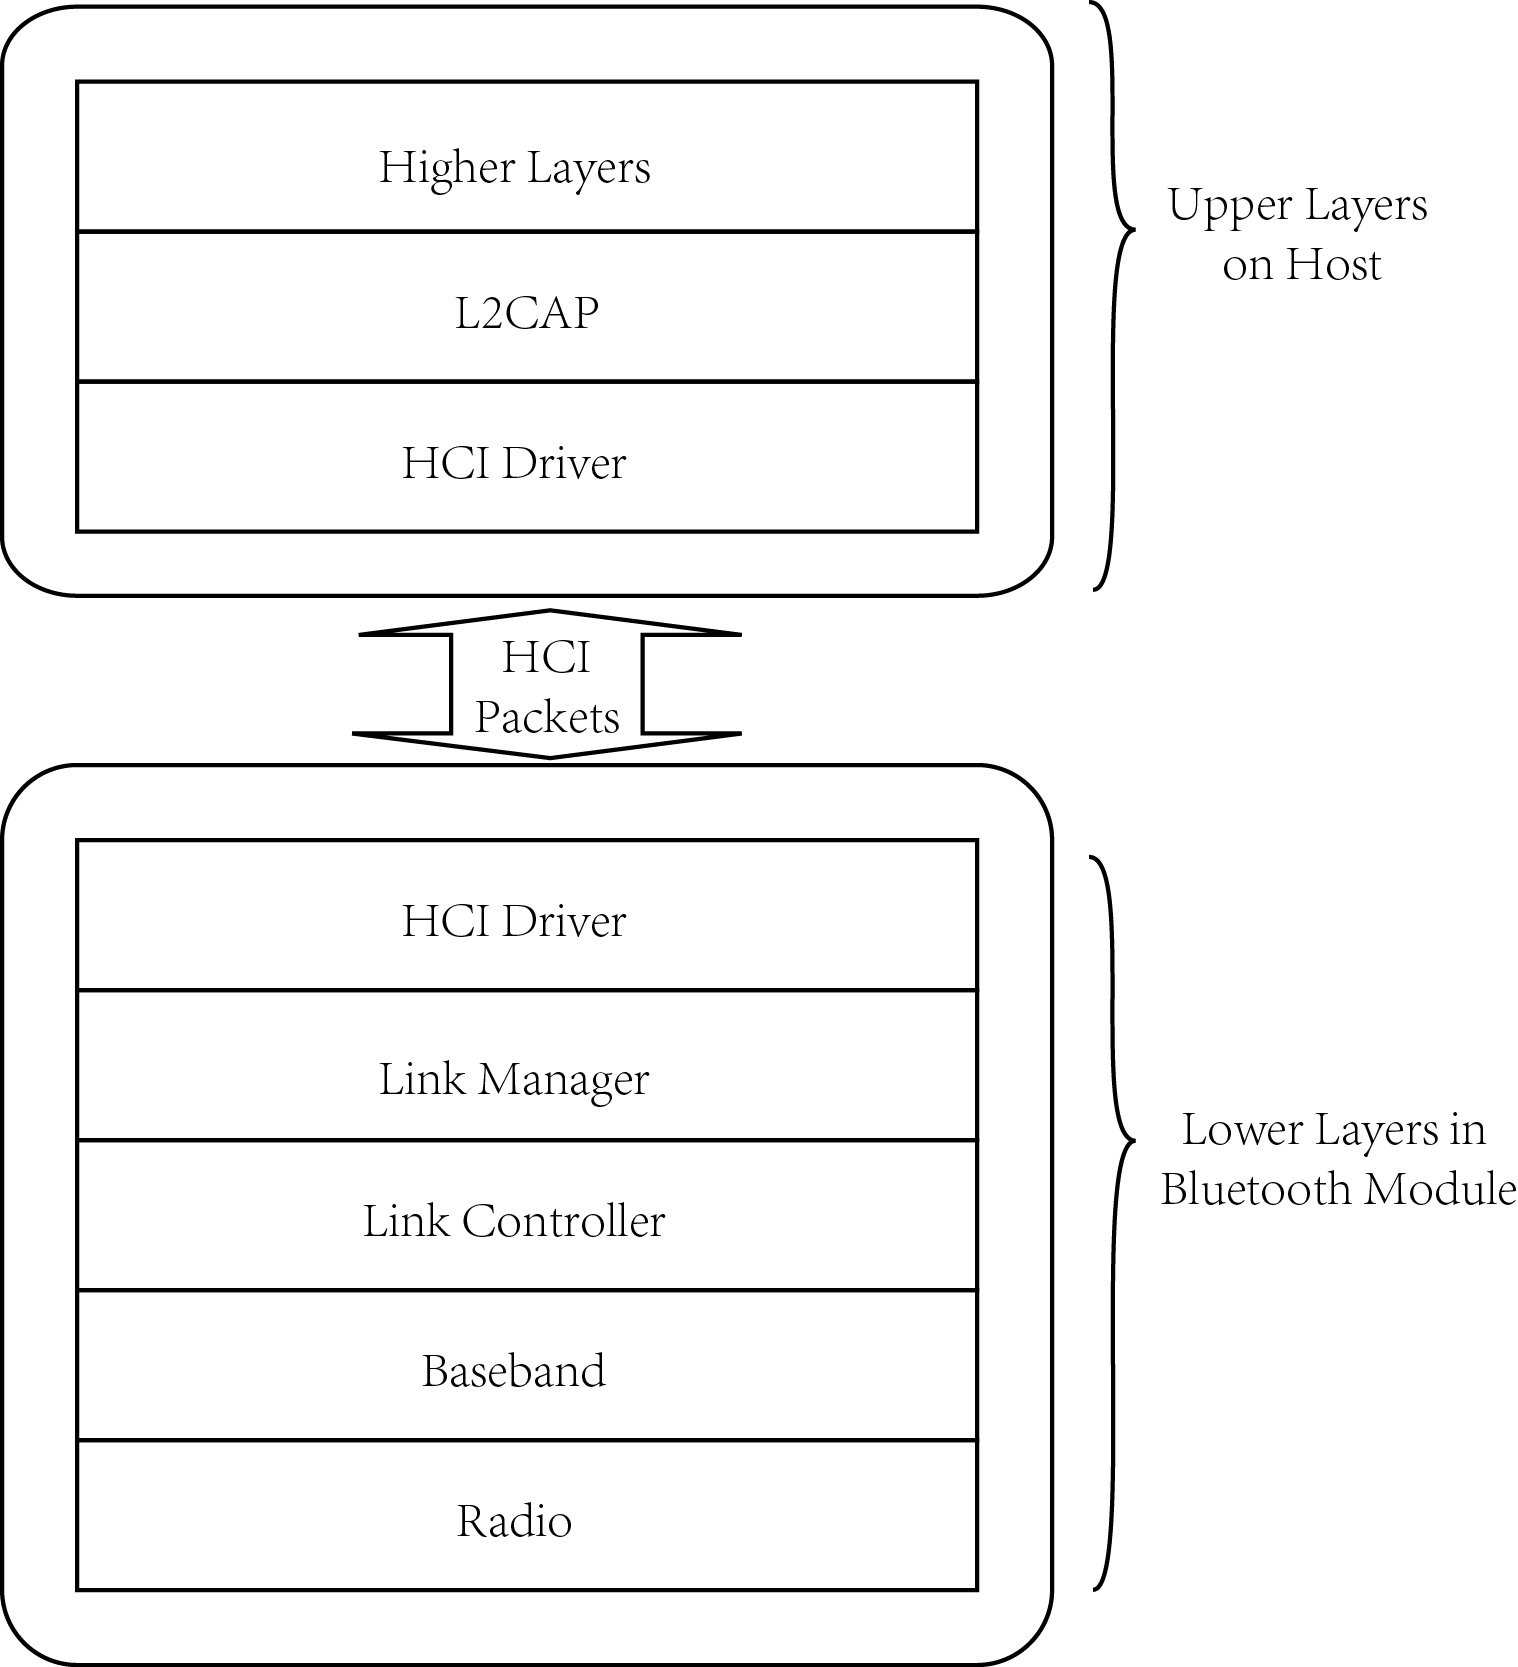
\includegraphics[scale=.7]{Figures/Figure4.png}
\caption{The HCI showing it's connection for the lower and higher level layers of the protocol}
\label{fig:HCILayer}
\end{figure}

Analogous to the transport layer in the OSI model, HCI provides a simplified interface to the Link Manager layer and is used connect to devices in proximity and manages its own transmission protocol packets. In order to facilitate the communication between the bottom and upper layers, this layer provides it’s own packet protocol that essentially are commands that propagate up, down, or in both directions between the interfacing and accessing layers. These packets include:

\begin{enumerate}
\item Command packets - sent from the upper layer to the lower layer to control the BT module and do things such as
    \begin{enumerate}
    \item accessing hardware registers
    \item setting up, tearing down, and configuring a connection
    \item changing power usage policies
    \item controlling baseband layer functionalities such as timeouts
    \item getting information about the host’s and other hosts hardware BlueStream needs to access and utilize these command during the execution of this service.
    \end{enumerate}
\item Event packets - sent from the lower layer to the upper layer to inform the host of changes in the lower layers, ie. callback after a command was completed successfully
\item Data packets - multi-directionality packets that facilitate passing contents of the BlueStream video frames up and down between the lower and upper layers    
\end{enumerate}

In contrast to the session layer of the OSI model, a connection between hosts are interfaced by the HCI layer, however the task is delegated to lower layers such as the Link Controller to physically make the connection. There is also some resemblance of the transport layer in the HCI layer since the packets of data that were broken up by L2CAP layer and are ready to be sent to the lower layers must be sequenced in the order that the data so the little packets can be reconstructed once again when it reaches its’ destination. There is a field for this sequence number in the HCI header. Another significance of this layer is the ability to send special inquiry command packets to enable the link controller to start the service discovery protocol and facilitate the result back to the upper layer to report the result back to the user. This protocol is initiated each time BlueStream looks for a device to send it’s screen capture to. During early stages of development, the developers of BlueStream had to log commands made by this layer to ensure that the right connection events and data transfer event were being called essentially making this layer the primary location to fetch the BT event history from. In summary, the HCI is an extremely important layer to the upper protocol stack layers as it abstracts a lot of complexity of the lower layer’s from the applications using BT technology. The layers above now resemble more closely with the application using this technology. Up next, it’s the L2CAP layer above HCI. 

\subsubsection{Logical Link Control and Adaptation(L2CAP) Layer}
Now that the description of the BT stack has reached the upper layers, it’s right to note that this layer and after are very close to the developers in such a way that it's possible to interface directly with them through code. The L2CAP is the first layer that allows that. This layer is the primary interfacing layer between the HCI and the RFCOMM above. In some devices, not Android, the HCI layer doesn’t exist therefore the L2CAP becomes the primary interface between the lower and the upper level modules. The purpose of this layer is to facilitate the packets transfer between RFCOMM and HCI layer. L2CAP provides a set of important functionalities to achieve this:

\begin{enumerate}
\item Acts acts a multiplexing layer using channel number as the demultiplexing key allowing higher level layer protocols such as RFCOMM to share resources provided by the lower level layer
\item Since lower layers require the use of smaller packets, like the baseband allows data segments of approximately 255 bytes, the L2CAP layer is in charge of segmentation of large data chunks that came from the higher level layers into smaller chunks for the lower layers. Conversely, the L2CAP layer is also in charge to reassembly of smaller chunks into the full payload (entire file) size. The L2CAP packet size is set to hold $2^{16}$ bytes and the large capacity is set in order to support the packet boundaries of the higher level layers.
\item Establishes asynchronous connectionless links
\end{enumerate}

\begin{figure}[h!]
\centering
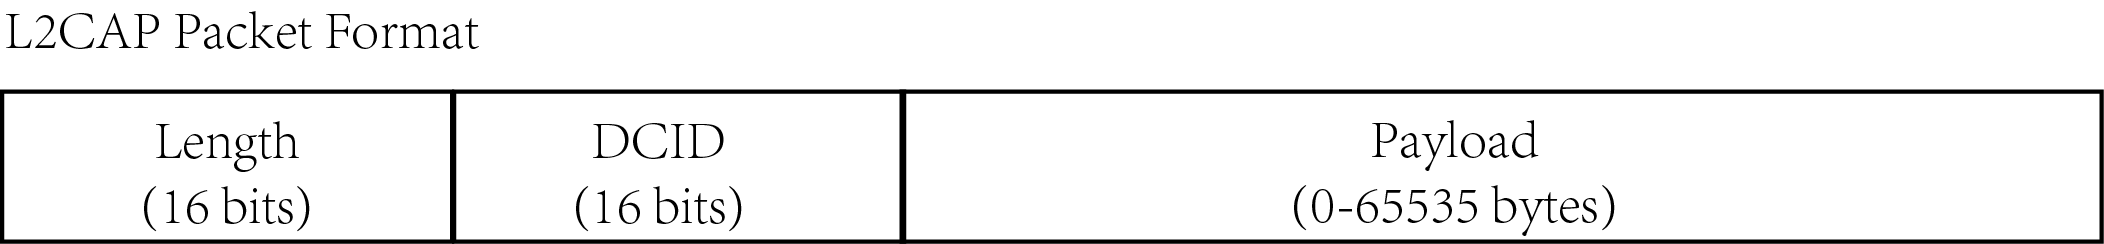
\includegraphics[scale=.8]{Figures/Figure5.png}
\caption{A L2CAP Packet}
\label{fig:L2CAPPacket}
\end{figure}

The interesting part of this L2CAP is it’s role in BlueStream and in the protocol stack. Up to know, the everything lower than the L2CAP is described in a way that depict each layer's functionality. However, the question remains, who initiates all those functionality? The answer is, some of those functionalities run on themselves such as power usage mode switches but most of the more interesting and useful functionalities are initiated by the user that interfaces with the L2CAP. Therefore, the L2CAP is here to:

\begin{enumerate}
\item Create connection requests - sending a request packet to the discovered device also running BlueStream
\item Request configurations of connecting devices - such getting other devices module version number
\end{enumerate}

After the connection is made stable, work is delegated to the lower level layer to listen for packets and send packets provided by the upper layers. The L2CAP layer plays a vital role in the BT protocol since all applications must use its packets to send data through to another device. This largely due to the ability for L2CAP to manage connection and segmentation of packets.Up next, a description of the RFCOMM layer and how it uses the L2CAP to bridge between the application and L2CAP. 

\subsubsection{RFCOMM Layer}
Fun fact, this layer emulates the RS-232 serial communication transmission port which was once was a standard long ago that connected printers, data storage, and even mice to early personal computers. This layer can provide multiple concurrent connections by relying on L2CAP’s ability to handle multiplexing over connections to multiple devices. In relation to BlueStream, this layer provides a simple and reliable data stream to the user. Since packet order has already been resolved in the lower layers, this layer emulates a bus for the bytes to travel through. The primary advantage of using RFCOMM is it’s wide spread support for legacy components and the APIs are very popular over many operating systems. In addition, the serial emulation provides an easy way to port devices who use serial ports as a medium to transfer data into RFCOMM. This layer is highly coupled with the L2CAP along side with the next protocol described. 

\subsubsection{SDP Layer}
In previous descriptions of lower layers, the term service discovery protocol (SDP) was mentioned. It was not mentioned what layer actually initiated this protocol, thus, the SDP layer around the same level as RFCOMM and also has tight coupling with respect to the L2CAP layer. Essentially as described before, SDP provides the means to find a device that BlueStream can connect to and stream to. The prerequisite for SDP to work is that two devices must be in range which triggers a link between the two devices. At this stage, only the L2CAP layer knows about all the links a particular device is connected to. Therefore, it’s up to SDP to go and find out about the services that the other device offers, such as a BlueStream device’s screen sharing service. When SDP returns with information about the configurations of the other device, the protocol hands off this information to the L2CAP layer and a separate connection is made to use that service. Once a connection has been made, two Android devices can both go into the “paired” state. This means that once SDP returned from its voyage with information about another device, it can store the MAC address of the other device into a SDP database for easy pairing next time the devices cross paths. This protocol also retrieves a 128-bit string ID called Universally Unique Identifiers (UUIDs), which identifies the type of service a device like BlueStream would offer. This UUID will tell all connecting devices that the services that the application offers is the screen capture streaming service. Further details of this protocol has been selectively left out as it deviates from the context of this report, there only the general idea was given about this layer. 

\subsubsection{Application Layer}
The application layer is the actual app that is running on user’s smart phones. This layer isn’t a real part of the BT protocol. However since by now, the full picture of the BT stack was described in previous sections, therefore it's time to put all these pieces together and explain how, from the developer of the app’s perspective, two Android devices can connect to each other. RFCOMM layer plays a very important role in connecting Android BT devices. The Android specific details for this layer has been retrieved from the Google android documentation\cite{DevelopersAndroid}. For two devices to be connected, it implies that the two devices share an RFCOMM channel. Alright there are two devices.

\textbf{Server S: } Let’s call device A for the server

\textbf{Client C:} Let’s call device B for the client

In order to connect our two devices, let S open a RFCOMM socket for the UUID for its service. When C and S get into range and C fires off a SDP. The SDP returns with the MAC address of S as well as the UUID. Remember the SDP protocol is used to retrieved information from all BT devices in your vicinity (10 meters) and the UUID is an unique identifier that marks the service that S can provide. If it’s the first time the two devices met, S and C will ask each other to accept each other’s information, which will be saved in a database so they don’t have to ask next time. Once both devices have accepted each other, their go into the connected state (their information passed down the layers and given link controller to manage the connection). Anything the client sends now the server can listen to.

Now let’s look at the connection from a client’s perspective. Suppose our two devices went home that night (and they live farther than 10 meters from each other!) and came back the next day. Now they want to connect. Since there exists an SDP entry for S in C, C can try to connect to S at any time, even when they’re are not within proximity. The matters of connection is a lot this time around. Since the SDP entry saved the device who provided the service with UUID, C can open a RFCOMM socket and ask server to also open one up. At this moment, a SDP request is fired of to S with a look up to see if they have a service that match the UUID that C is requesting. If S does, then S answers C by opening up its own RFCOMM socket to connect to the client’s channel, then the connection is established. If anything wrong happens during this phase, a timeout of 12 second will instantly throw an exception. 

This wraps up the BT protocol from the Radio layer to the Application layer. Up next, the background in the stream technology is explained.

\subsection{Motion-JPEG Video Compression Format}
The main technology used for the streaming behaviour for BlueStream is the M-JPEG is a video compression format. Developed by QuickTime in the early 1990s, this format was carefully selected for it’s simplicity, stability, and flexibility over other formats that tried, tested, and failed. Unfortunately, there isn’t an official specification document so the information obtained to write this section had to come from Wikipedia \cite{MotionJPEG}. M-JPEG was once first popularized by the PlayStation and Nintendo Wii consoles. More recently, Apple has announced the support for M-JPEG in their new AppleTV. So exactly is BlueStream using M-JPEG?

M-JPEG utilizes the intra-frame compression method, meaning each individual frame is compressed separately from the whole video. Each frame, as you may guess, is actually comprised of a JPEG image and with a stream of images. Figure \ref{fig:MJPEG} roughly sketches how this is done from one device to another. The idea behind the streaming functionality of BlueStream, is to transfer a constant flow of images from one device to another. Compared to other formats, M-JPEG used more space, however the nature of the stream does not allocate any persistent data, thus, would not result in a situation that fills up the viewer’s memory of irrelevant frame data. By capture images from one device’s screen as fast as possible, it allowed development to use the built in tools and libraries of the Android ecosystem providing the provide a dash of simplicity. Failing to capture a frame does not corrupt the frame similar to how UDP works. The frame serving device sends over as many frames as possible and if some are corrupted or lost on the way, the viewing device simply skips a frame providing a real sense of stability across the BlueStream. Performance of the application relies on the speed of the frame transfer and as well as frame decoding. With that said, the intra-frame compression methods provides BlueStream the ability to set the quality of the video which will have an effect on the frame rates. We used an open source library made by neuralassembly \cite{SimpleMjpegView} to facilitate decoding and deserializing the frames arrive at the viewing device. Lower quality means smaller frame sizes and in turn means, more frames per second. More of this will be described in the result and evaluation section. 

\begin{figure}[h!]
\centering
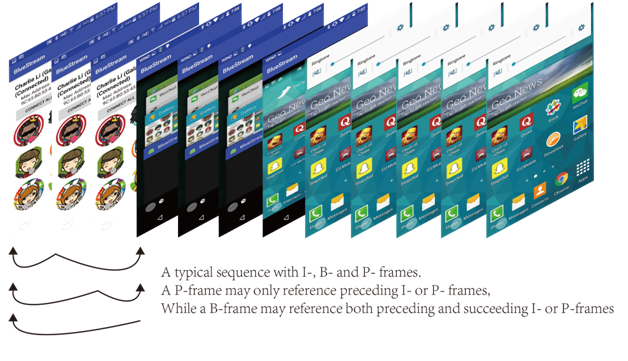
\includegraphics[scale=.7]{Figures/Figure6.png}
\caption{Depicting of how inter-frame compression works in respect to a stream, each frame is compressed individually}
\label{fig:MJPEG}
\end{figure}

This concludes the background section of the BlueStream technologies. This section will be constantly referred to as some of the important layers of the protocol explain the reasons behind the performance of BlueStream and its limitations. The next section will begin formulating our test data for the application and show the performances of the application under different settings.

\section{Result}
The resulting application from the hard work from the members of the BlueStream team is outlined in this section. Focus has been drawn toward the application design and architecture of the application and will provide the reader with a summary of the design choices made at each step of the application development. The core algorithm for the stream behavior is explained in detail that encompases each step of the frame transfer between two connected devices. Results for the BlueStream benchmark tests have been depicted graphically for the reader to follow and an explanation of the test scenario will be given for each graph. Each graph will have a purpose in recording the behaviour, performance, and values obtained from external factors such as the distance between the linking device, the processing time of the algorithm, signal strength, and the size of the frame being transferred. The purpose of these graphs will generally be used to determine its effect on the performance of the algorithm and design of BlueStream, hence, leading to the first section to be covered, the design and architecture.

\subsection{Design and Architecture}
BlueStream was carefully designed to extract the maximum performance and functionality of the Android API $>$ 5.x. Due to the well integration and support for BT in Android, development only had to focus on the high level application layer of the protocol. Our team developed design goals for BlueStream as follows:

\begin{enumerate}
\item Design Goal 1 - \textbf{Performance} - Application must implement the fastest, measurable frame per second over a screen sharing stream. 
\item Design Goal 2 - \textbf{Reliability} - During runtime, application should not crash unexpectedly and handle cases where disconnections may happen. 
\item Design Goal 3 - \textbf{Flexibility} - Code written should be decoupled within the architecture of BlueStream for easy reuse and extensibility.
\item Design Goal 4 - \textbf{Usability} -  BlueStream will strive to design the user interface to be easily used by the general public.
\end{enumerate}

Through these defined design goals, the application development began under the Android platform. Below Figure \ref{fig:UML} depicts the entire UML class diagram is included for the BlueStream application. For simplicity, multiplicity has been left out and only associations are drawn for each relationship of the class. The main activity that hosts the entire BlueStream application is located bottom center, above the title. The architecture for Bluestream is designed for P2P connection. Please refer to the diagram and a description of the subsystems will be described after.

\begin{figure}[h!]
\centering
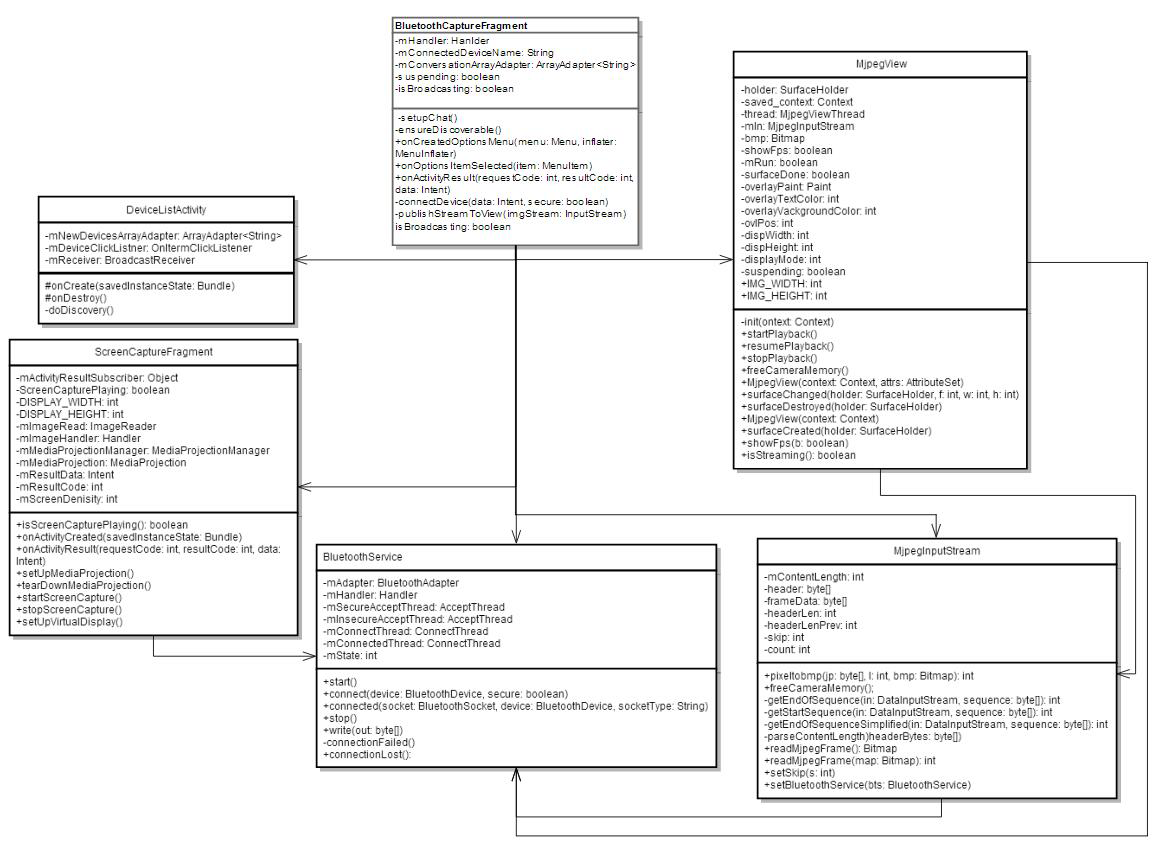
\includegraphics[scale=.5]{Figures/Figure7.png}
\caption{The UML diagram of BlueStream and its architecture}
\label{fig:UML}
\end{figure}

The subsystems that comprise BlueStream are: \textit{ScreenCapture}, \textit{BluetoothCapture}, \textit{BluetoothService}, and \textit{Mjpeg}. A description of each subsystem will follow.\\

\noindent \textbf{ScreenCapture subsystem} - This subsystem is used to encapsulate recording behaviour. This subsystem provides the functionality to enable/disable recording, capture individual frames from the device screen, and compress and resize each frame to provide for the BluetoothCapture subsystem.\\

\noindent \textbf{BluetoothCapture subsystem} - This subsystem is important to facilitate the initiation and teardown of a connections between two devices. The primary functionality of this subsystem is the control a live connection, manage frames to be sent, and manage frames to be received. The functionality is similar to an overall BlueStream controller that depend on the \textit{ScreenCapture}, \textit{BluetoothService}, and \textit{Mjpeg} subsystems.\\

\noindent \textbf{BluetoothService subsystem} - This subsystem is used to abstract the complexities of connection to another device and resource allocation to manage the connection in a separate thread. Its job is to includes device discovery, device connection, connection tear down, and error handling. \\

\noindent \textbf{Mjpeg subsystem} - This subsystem is in charge of reconstructing a stream of frames provided by the \textit{BluetoothCapture} subsystem. Its job is to convert the byte stream of frames back to a viewable image and display it through the \textit{MjpegView} class. \\


As of now, both design goals and subsystems of BlueStream has been defined. The rest of this subsection will describe the intersection of design goals and architecture. The primary design goal for performance was thoroughly considered over the course of the development phase. Through use of the built in image viewer class of the Android API, the development team deemed the performance too crude and slow. In order to engage the high level libraries contained in the API, the development team opted to implemented and link native low level C libraries to deserialize the byte stream back into a viewable frame that the \textit{MjpegView} class can display. 

Challenges to managing a BT connection was a big challenge during development and a solution was provided by abstracting the BT connection logic to the \textit{BluetoothService} subsystem. Connections are encapsulated within the \textit{BluetoothService} class and when one device is gone out of range or manually disconnected, this subsystem will throw an exception and terminate the stream without crashing the application. This abstracted also aided in the performance design goal as the a seperate thread handles the connected devices and channels data between them. 

The design goal 3 for flexibility is performed by lowering coupling between each subsystem. Using a controller subsystem \textit{BluetoothCapture} in the P2P architecture, the interfaces of the other subsystems are collected then their services utilized. This subsystem primarily connects the \textit{ScreenCapture} with the \textit{BluetoothService} subsystem in order to feed frames to the BT socket when the device is in recording mode. Conversely, \textit{BluetoothCapture} also connects the streams between \textit{BluetoothService} and \textit{Mjpeg} subsystems to allow frames received through the BT socket to be displayed. Through this design, the subsystems of BlueStream become modular which leads to a plethora of software engineering benefits.

\subsection{Stream Algorithm}
This following section will depict the stream algorithm in detail. The main purpose of the algorithm is to maximize the number of frames the recording device can capture and send over the wireless connection. Description for the algorithm will begin with the recording device and end at the receiving device. For convenience, the algorithm will be descripted as a flow of events from the recording device to the viewing device. 

\textit{Algorithm preamble}: two devices are connected through BT and are running BlueStream application. One device selected the option to record it’s screen and is prompted for security permissions access. The user will allow BlueStream to access the device’s screen information, and thus, the algorithm for screen capture begins with the recording device capturing an image. See Figure \ref{fig:FrameSeperation} for an illustration.

\begin{enumerate}
\item An image reader is created that listens to the screen for any change. When the picture on the screen changes, an event is fired off to notify the event handler that the screen changed.
\item The event handler is called and takes a snapshot of the current state of the screen and converts it to a generic image object. 
\item The image is handed to the image processor where the dimensions of the image (of the screen’s state) is determined.
\item The generic image object is then converted to a byte buffer for modification.
\item The new buffer is processed by the Bitmap class, where the raw bytes are converted to ARGB (alpha, red, green, and blue) format. Each pixel of the resulting bitmap becomes a 4 byte size. 
\item The resulting image buffer is now the raw 1920x1080 image that the screen captured. The size of this image makes it infeasible to attain a viewable frame rate, therefore, must be processed. 
\item A sweet spot was found for frame size 640 pixels height and 480 pixel wide. Also a compression of 50\%. Due to the nature of JPEG format, compression is always in a lossy format. Therefore the resulting image after compression will be significantly decreased in size (and unfortunately quality loss as well).
\item The compressed, resize image buffer is sent to the output stream in the BluetoothService subsystem written to the socket where it is transmitted to the receiving device.
\item Repeat step 1 until disconnection or stream abort. 
\end{enumerate}

When the sending device received the full buffer that the recording device has sent, the following happens:

\begin{enumerate}
\item The \textit{BluetoothService} passes the input stream directly to \textit{MjpegView} and a buffer will be started to fully collect the packets from the BT transfer (since it’s heavily fragmented at the baseband layer). 
\item Once the input buffer is full, the header of the byte stream is searched to verify the buffer contains a valid JPEG header. 
\item The input stream buffer is copied into another temporary buffer to release the resources of the input stream in order start accepting more frames while processing the received buffer. 
\item The temporary buffer is sent to the native bitmap processing library where it is converted to an JPEG image.
\item The viewer surface now displays the JPEG image on the screen then step 1 repeats if the input stream becomes full again.
\end{enumerate}

\begin{figure}[h!]
\centering
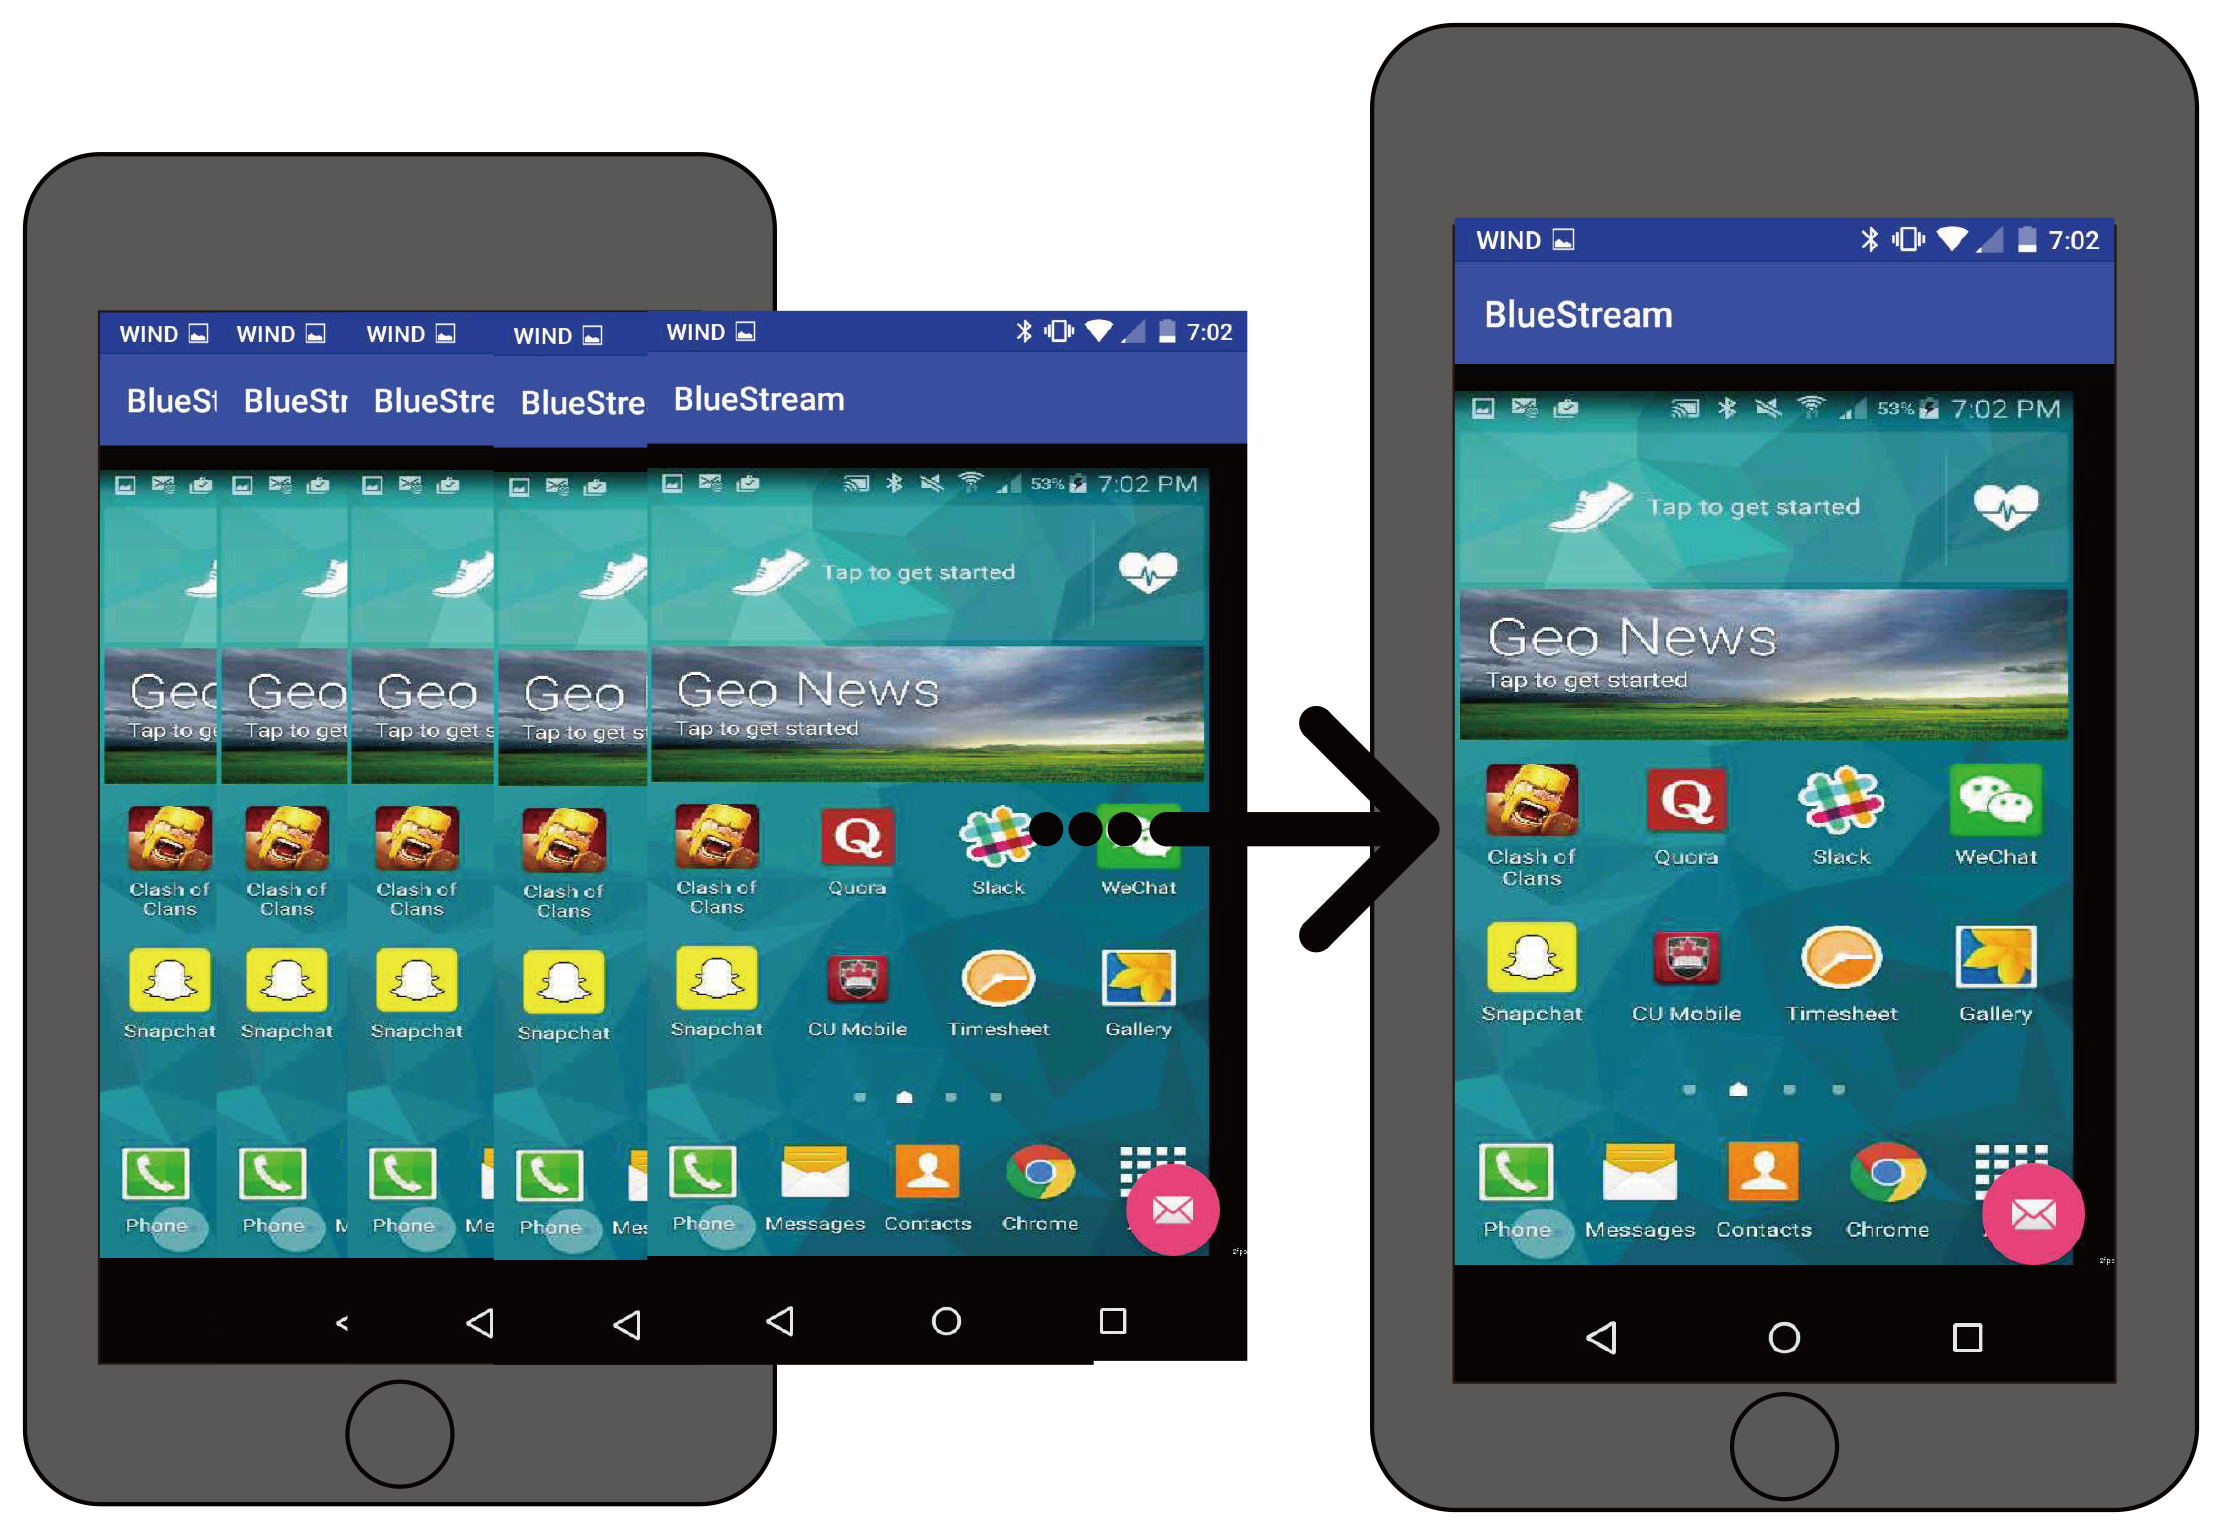
\includegraphics[scale=.5]{Figures/Figure8.png}
\caption{A diagram showing frames being transferred using a buffer from one device to the other}
\label{fig:FrameSeperation}
\end{figure}

\subsection{Performance Benchmarks}
After BlueStream was completed, it became the utmost importance to validate the performance of the application. The team wanted the best performance out of the stream algorithm and always asks the question: “can we do better?”. The object of this section is to show the performance metrics of BlueStream in a measurable characteristic of frames per second and determine the bottlenecks of the application to improve on. The results of this subsection will be referenced and analyzed for the next section, Evaluation. In this section, the performance of the application is measured under multiple external environment influence factors such as distance, processing time, image size in relation to quality of compression, and signal strength. Each paragraph will explain the environment that the influences are tested under starting with the distance. Over the course of the report, the term “compression” is mentioned many times, however, in this section the compression is referred to as quality rate where a higher quality rate means a lower compression ratio. The following experiments were recorded during a streaming session where the subject device (recording device) had played a ~30 second movie clip to another phone.

\begin{figure}[h!]
\centering
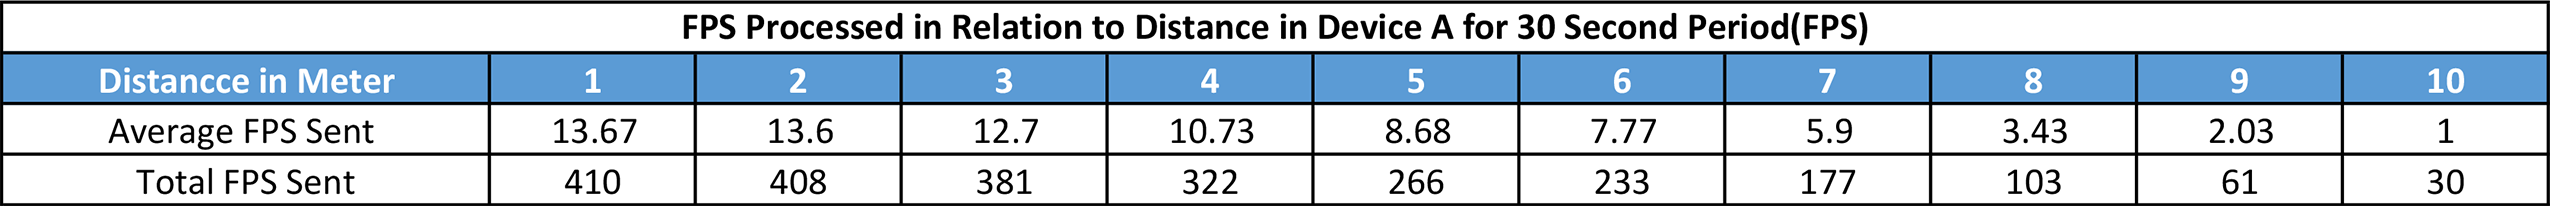
\includegraphics[scale=.7]{Figures/Figure9.png}
\caption{Frame per second transferred over the distance between the two devices}
\label{fig:FPSoverDistance}
\end{figure}

Figure \ref{fig:FPSoverDistance} shows the change in frames per second over the distance of the connected devices. Raw data for this experiment was included and averaged from Appendix 3 and compiled into an average. This experiment was done by measuring a 10 meter distance between the recording and receiving device with a preset quality level of 20. Within each interval of distance, a 30 second clip was played to the viewing device and the average frame rates recorded at each interval. The table draws some interesting facts about BT and it’s ability to transfer data across distances. From Figure  \ref{fig:FPSoverDistance}, a slow decrease in frame rate is visible when the distance of the devices start drawing farther and farther apart. Nearing the the 9 meter mark, the stream becomes very choppy and is nonviewable. By the 10th meter, the stream is cut off totally. This behaviour was expected from class 2 BT devices as the transfer distance is capped at 10 meters. Up next, the average frame size in kilobytes is shown from the result of the quality ratios applied during the algorithm

\begin{figure}[h!]
\centering
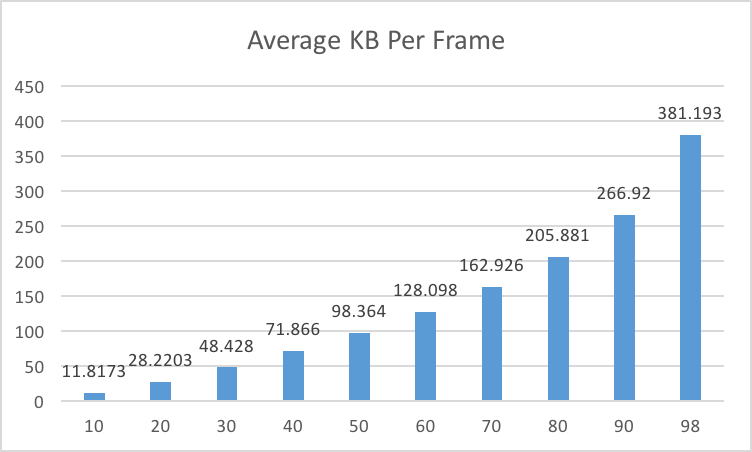
\includegraphics[scale=1]{Figures/Figure10.png}
\caption{Average frame size resulting from each quality rate applied}
\label{fig:AvgFramesQuality}
\end{figure}

Figure \ref{fig:AvgFramesQuality} shows the size of each frame after the algorithm has applied the compression relative the the image quality that’s set. This size is the physical frame size of the JPEG frame that will be sent over the network. Raw data for this experiment was included and averaged from Appendix 4. This experiment was done by diverting the image buffer gathered from a single screen capture from being sent over the link and instead, to be saved on internal persistent memory. The experiment was repeated 30 times within 1 meters distance for each quality rate (10 to 98) and the average size of the images in kilobytes were recorded. This data shows the size of each frame is a function of the quality ratio as image quality is increased, the size of the transfer is also increased. Due to the size of the image buffer in the MJPEG library we used, a full image quality value of 100 could not be used in order to avoid an occasional buffer overflow. From this data, we can conclude the range of sizes for lower and higher quality frames to be sent over the screen. Up next is an investigate to find correlation between the frame rate and the sizes that were discovered. 

\begin{figure}[h!]
\centering
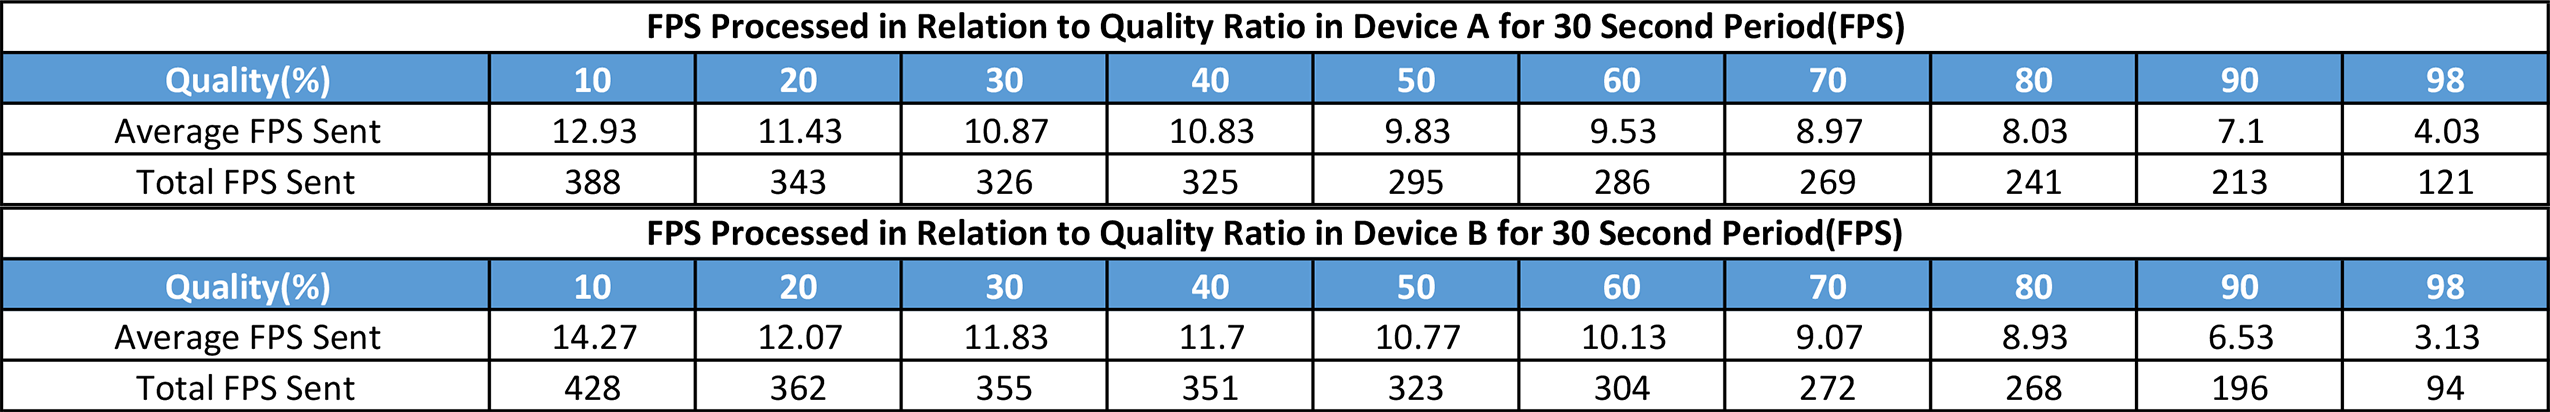
\includegraphics[scale=.7]{Figures/Figure11.png}
\caption{Frames per second in relation to processing time of test device A and B}
\label{fig:FPSprocessingTime}
\end{figure}

Figure \ref{fig:FPSprocessingTime} shows the change in frames per second over the different processing times for the two test devices A and B. Raw data for this experiment was included and averaged from Appendix 1 and Appendix 2. This experiment was done by switching the roles of receiver and recorder between devices A and B to record the amount of fps each device can process. This experiment was done by streaming a 30 second clip at 10 different intervals of quality rates at within 1 meters distance between the devices. The quality rate is defined as the amount of compression our algorithm will apply to each frame and is a measure to the extend of lossy quality in each JPEG frame. A general guide to making sense of the quality value is defined as a range from 10 to 98, where 10 is the lowest quality (most compression) and 98 is the highest quality (almost no compression). From the results we can clearly see that the quality of each frame plays a huge factor in the performance of the screen recorder in our peer to peer model. 

\begin{figure}[h!]
\centering
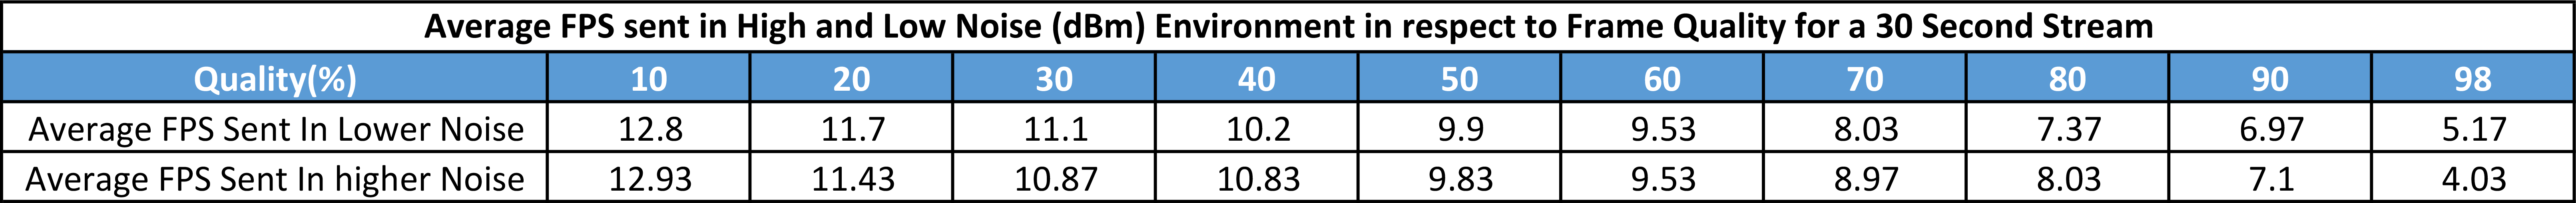
\includegraphics[scale=.285]{Figures/Figure12.png}
\caption{Average frames per second during high and low noise environments}
\label{fig:FpsNoise}
\end{figure}

Figure \ref{fig:FpsNoise} shows the effects of frame per second over two connections experiencing varied levels of noise which negatively impacts the signal strength of the connection. Append 7 shows the raw data for this experiment. This experiment was conducted throughout Carleton by using a spectrum analyzer application to determine areas of high and low noise. We found areas of the senior undergraduate lab to have high noise within the 2.4-2.5GHz spectrum while areas like the Carleton underground tunnels had low noise within this spectrum range. The connection was initiated less than 1 meter away from each device.

\section{Evaluation}
This section is dedicated to the evaluation of BlueStream’s performance characteristics by beginning with a description on our analytical model. In order to properly evaluate the performance of BlueStream, we have selected frames per second (FPS) as the primary indicator of performance in our model and will be used as a comparison factory throughout this section. The position we choose to take in this section will evaluate the performance by comparing the data for FPS that is collected from Section 3 to find out what settings are best used to optimize the performance of the streaming algorithm. We will begin by informing the reader about the maximal theoretical and practical data transfer rates in the subsection The Possibility Challenge to explain the wireless technology can obtain in order to get a good foothold on the performance constraints that BlueStream has encountered. Thereafter, the subsection pertaining Our Data will portray the highest resulting data transfer rates that BlueStream can obtain in a perfect practical scenario to measure the proximity in relation to the maximum transfer rates. Lastly, the Environmental Factors section will consider the different  causes which affects the performance of BlueStream. The data mentioned in this subsection include the data we collected from our self experiment, shown in section 3. In conjunction with the evaluation, the goal is to identify a quality level we set for BlueStream that can maintain a stream at a level of good performance as well be usable when confronted with various environmental disruptions. In the end of this section, we will put our conclusions to the test by surveying fellow peers on the app’s optimal performance settings. 

\subsection{The Possibility Challenge}

In order to properly evaluate how well BlueStream performs, a point of reference must be established. The goal of this subsection is to identify an upper bound on the performance of BT wireless technology and show the impossibility to perform better than this level. The final product of BlueStream aims to reach this goal in close proximity however it most likely infeasible as a variety of external factors will come to play as explained in the \textit{Environmental Factors} section. Since Bluetooth is already on version 5.0 at this date of the report, the test device used during the development phase were equipped with 4.0 version and were not using the lighter low energy edition. The functionality of BlueStream is to send frames across the wireless link so we will compile rough sketch of the size of each frame that we are hypothetically working with.

The recording all happens on a 1920x1080 pixel screen with each pixel containing 32 bits of color (8 bits for R, G, and B, and then last 8 for the alpha channel). Since each pixel is 4 bytes, and the total amount of pixels in each frame is $1920\times 1080 = 2,073,600$, then the size of this raw image would be$ 2,073,600\times 4 = ~8.3Mb$. In order to use the M-JPEG compression, we must reduce the frames from here to 640x480 dimensions, which the new raw image size is ~1.2Mb. Since zero compression will blow out the buffer for the MJPEG plugin, a compression is necessary. Suppose we use 10:1 compression ration, then the resulting image size is 122Kb which is roughly a quality ratio of 60 that can be set in BlueStream. Let this image size be our point of reference for this section.

Many media outlets boast such as the one by GizMag, they say BT after version 3.0 can attain a data transfer rate of 24Mbps \cite{GizMag} since the support came from the 802.11 protocol adaptation layer. If this is the case then the following formula will describe the maximum number of frames possible with the current configurations.

$$FPS = \frac{24\frac{Mb}{s}}{122\frac{Kb}{frame}} \approx 196$$

This is rather impossible since the our data showed that the maximum number of NULL frames was 50 to 60. Now let’s consider actual data transfer rate posted on the Bluetooth technology website. The article on “What is bluetooth” <cite> shows that the gross air bit rate is 2Mb/s, far from the 24 Mb/s that media outlets were claiming. With this transfer rate, we repeat the calculation for the expected frame rate.

$$FPS = \frac{2\frac{Mb}{s}}{122\frac{Kb}{frame}} = ~ 16 $$

That data is is quite in line with the data collected and puts in a more realistic perspective into the maximum performance of BlueStream. An interpreted reason for the high difference between the actual air data transfer rate versus the claim 802.11 is due to the segmentation of packets being sent through the wireless link. The bluetooth protocol segmentates packets at high rate in order to fit the transfer size within the frequency hop windows to prevent interference with other radio signals. Hewlett Packard published an article comparing Bluetooth and WiFi in 2002 and compared the two protocols in detail. The take-away from that article was that BT and WiFi, even operating under the same adaption layer, are equipped with different technologies. WiFi uses a different spectrum hop mechanism called direct sequence spread spectrum that allocates one channel the size of 22Mhz wide. Comparatively speaking, 22Mhz is much larger than BT’s 1Mhz channel, thus, allowing higher bandwidth on the transfer. 24Mb/s is now made clear as unattainable transfer rate as we speak about the performance of BlueStream. The target of this application to attain 16 frames per second without consideration of some external factors that may hinder this bound. The next section will investigate the data we collected in contrast with the maximum frames per second upper bound. 

\subsection{Our Data}

The data we recorded during the performance benchmarking of BlueStream did not come as close as anticipated to the upper bound of transfer. During our experiments a image quality of 60 allowed a close representation of the 10:1 compression ratio used on each frame of the stream. The average size each frame, captured over 30 seconds, was 128 kilobytes as indicated in Figure \ref{fig:AvgFramesQuality}. The average frames per second, captured over 30 seconds, was 6.2 fps as shown in Figure \ref{fig:FPSoverDistance}. That’s a dramatic 10 fps less than the cap. Figure \ref{fig:AvgFPSdistance} shows the average data rate for each preconfigured image quality ratio. The last row shows the number the data transfer rate at each quality interval.

\begin{figure}[h!]
\centering
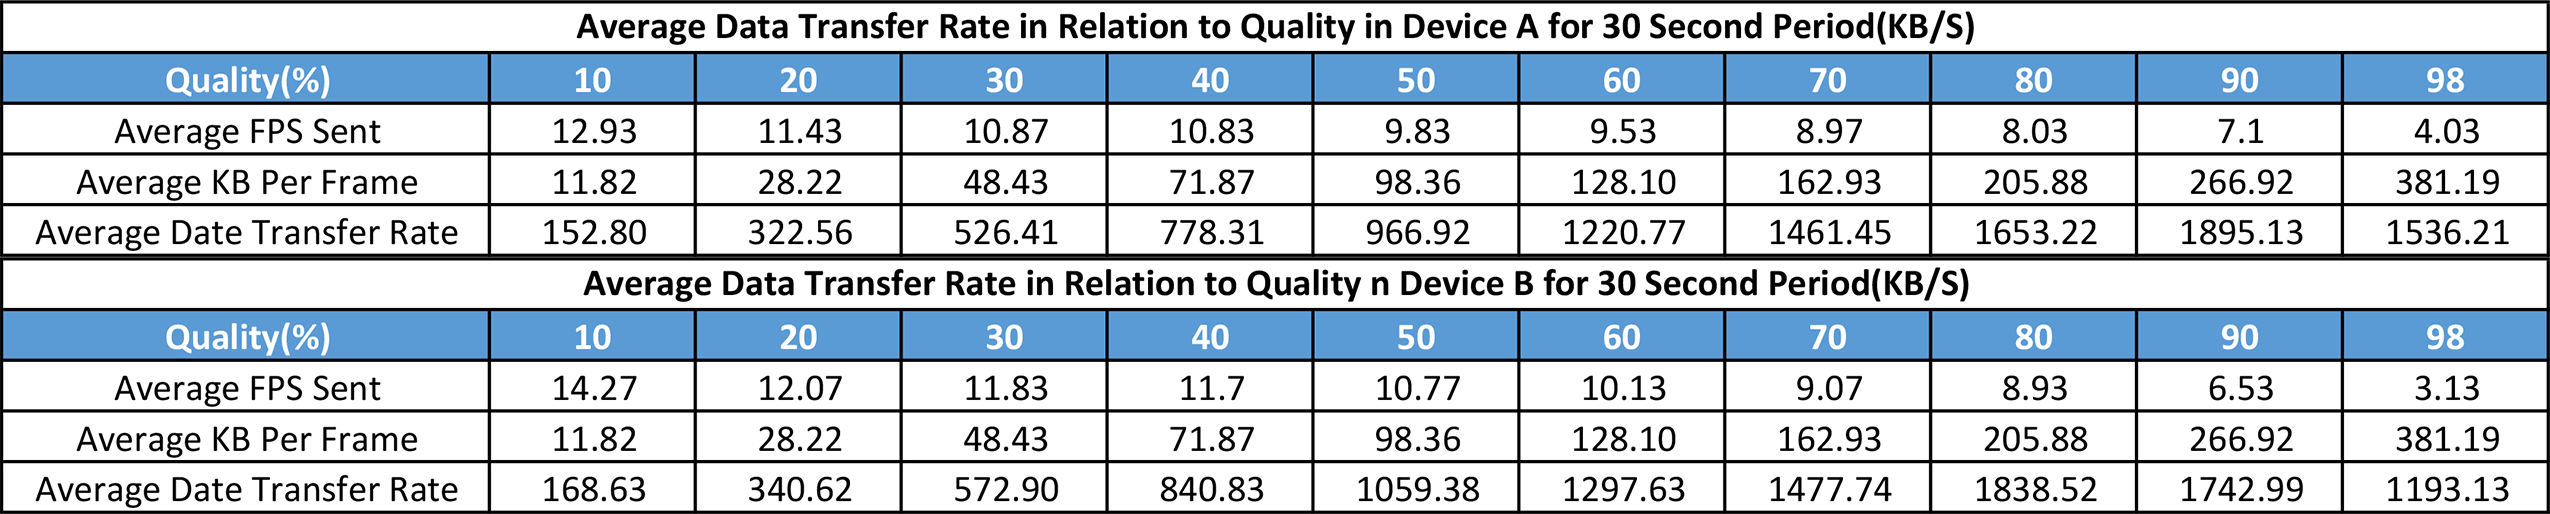
\includegraphics[scale=.7]{Figures/Figure13.png}
\caption{Average FPS in relation to quality set for Device A \& B}
\label{fig:ScalingDimension}
\end{figure}

As the data indicated in Figure \ref{fig:ScalingDimension} the a peculiar pattern emerges. The comparison between high quality versus low quality frames BlueStream produces show an inverse relationship between FPS and data transfer rate. This data implies the data rate is very fast when transferring chunks of data (frames) and is lower when sending more smaller chunks. In the algorithm described in section 3, we have defined 3 constants that may affect the recording device’s packaging of frames. Why we are only concerned primarily with these constants because the experiment was performed in the “best case scenario” environment based on other factors we determined, such as noise, distance, and signal strength. The constants includes taking a snapshot of the current screen’s state, JPEG compression, and serialization of the data. If we assume these three constants as the cost of capturing a frame, we can draw a conclusion toward the cost of this constant is high. When the frame rates increase, the cost for capturing frames over shadows data transfer limit of the link. Conversely, when the frame sizes are large in a quality value of 90, each image consists of a large chunk of data to be packaged into the L2CAP layer. We can utilize nearly the full bandwidth of the BT link nearlying ~1.9MB/s while suffering an approximate frame rate of half. 

In the best case scenario, we have found that the main internal bottleneck of BlueStream is actually the processing capture time. This factor is broken down into serialization, JPEG compression, and image capture. We shall analyze which of these factors have the most influence. Serialization is a linear operation and is always fast as it process images at the bit level to package them into an array of bytes for the L2CAP layer to be fragmented and passed down the layers. The high data rate for larger images show that this movement of data from top to bottom layer is fast, which constitutes the high data rate for low frames per second. How about JPEG compression? According to D. Finell, D. Yacoub, and M. Harmon in their paper \cite{JPEGCompression}, the JPEG compression algorithm runs in $O(n^2 logn)$. The runtime may not scale completely find into a large n into the millions, but should be quite a fast operation when operating on 640x480 images. The last constant factor is the capture mechanism for each frame. As we ruled out the other two factors, it seems self-evident that capture video frame by frame is the high run time component of the algorithm. We inspected the Android source code to find some clues to why this section of code is the slowest and found that the producer-consumer paradigm is used for the reading each frame off of the screen. In this method, the production of individual frames in a buffer is slower than availability for the consumer to process and send the frames over a network.  
    
In order to explain the differences between the upper bound and our result, our investigation examined the different external factors that can impact the performance of BlueStream in a non-perfect environment. Several factors that influenced the FPS were considered including distance between the connected devices, the amount of noise that can affect the signal of the connected devices. 

\subsection{Environmental Factors}
This section will raise a discussion on the possible external factors that can degrade the performance of the stream. It's important to note that these factors are generally uncontrollable by the end user, however will provide a convincing argument to define what settings we select for BlueStream as being optimal. For instance, we saw in the results section that the FPS decreases as a function of the distance between the recording and viewing device, there setting the quality level too high hinder the usability of the application. We will start off by showing the most common factor that user will experience when using our application, the distance between the two connected device.

\begin{figure}[h!]
\centering
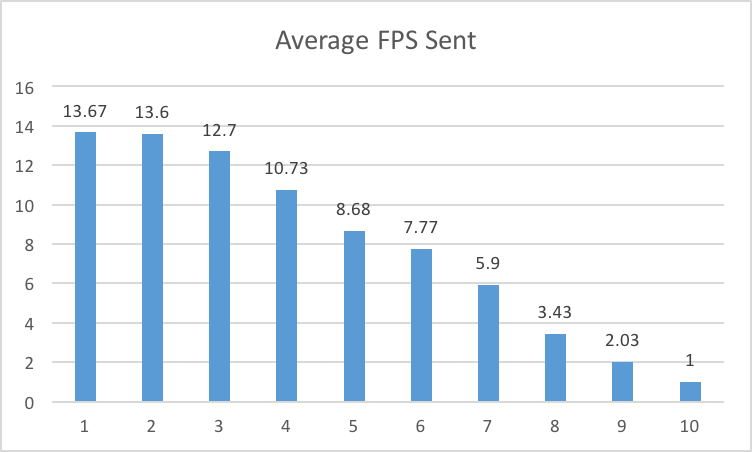
\includegraphics[scale=1]{Figures/Figure14.png}
\caption{Average FPS received from the stream across 10 meter distance}
\label{fig:AvgFPSdistance}
\end{figure}

We’ve all experienced low connection speeds around Carleton before, so the results from our test to benchmark FPS in terms of distance came to no surprise. Just like the hindered performance of internet packets arriving at the host machine, BlueStream’s affected by the slow of packets in the same way. Since we mentioned Bluetooth packets are significantly smaller than internet packets as described in Section 2, a slight delay per packet can aggregate into large amounts of downtime. This result of this delay implicates a degenerated performance level for BlueStream, as its unable to send frames of its stream in a fast low latency way. The question that this raises is, where do the excess frames go if the streamer is still producing more frames than the consumer can take in? The answer lies in the Baseband layer and it’s asynchronous connectionless link \cite{BTUnifyingTheTelecom}. This connection protocol is similar to TCP where the contents of its data is more important than latency, and hence, will make sure the entire frame is completely received before accepting another one. The viewing device spends a longer time putting the frame packets back together than the streaming device at packaging the frames therefore, the frames that are sent in between the reconstruction time for a previous frame on the viewer are lost or dropped. This explains the the decrease in frame rates over an increase distance between the link. Over this distance, the reason for slow-down is the weakening of the signal. The following figure will show the signal strength between two connected devices.


\begin{figure}[h!]
\centering
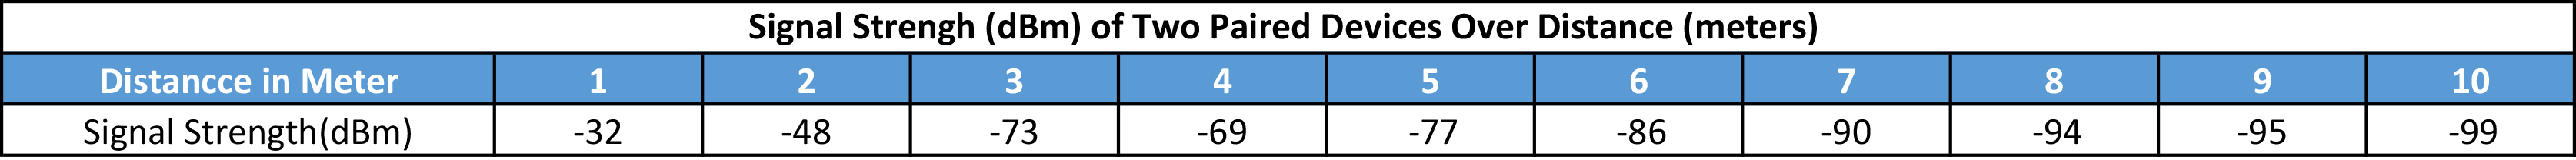
\includegraphics[scale=.55]{Figures/Figure15.png}
\caption{Signal strength in relation to distance}
\label{fig:SignalStrength}
\end{figure}

Figure \ref{fig:SignalStrength} shows the signal strength of two BlueStream devices as the distance between them increases. We can see that the signal strength deteriorates at a rapid level. In order to make sense of this data, we calculated the data transmission speed in relative to the distance as we now know the signal strength gets weaker as the distance between the two devices increase.


\begin{figure}[h!]
\centering
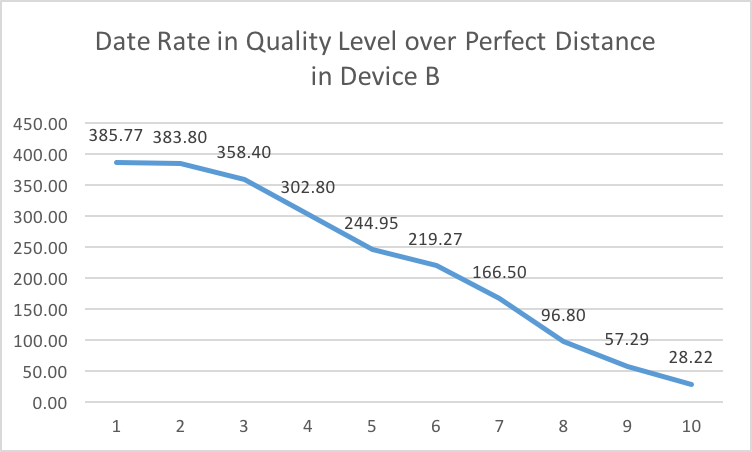
\includegraphics[scale=1]{Figures/Figure16.png}
\caption{Data rate(KB/s) of the stream in relation to the distance and quality}
\label{fig:DataRateDistance}
\end{figure}

The graph above shows the degrading transfer rate as distance between the two devices increase. This experiment used the average FPS taken from Figure \ref{fig:FPSoverDistance}, across an interval of 1 meter, to show the data rate of the size of a frame at a quality level of 20, showing in Figure \ref{fig:AvgFPSdistance}. Essentially the figure \ref{fig:DataRateDistance} shows the data rate to transmit a 28 kilobyte image frame over 10 meters. This data proves that distance, the strength of the signal actually has a big impact on the performance of BlueStream. The data we collected for this graph makes sense because the strength of the signal refers to the magnitude of the electric field at which a device is transmitting at. More power actually increases the amount of information that can be transmitted through the link. This brings up an interesting question about other effects that could deteriorate signal strength, hence, the performance of BlueStream. Next we investigate we whether noise is a big can cause a big interference of our connection.

\begin{figure}[h!]
\centering
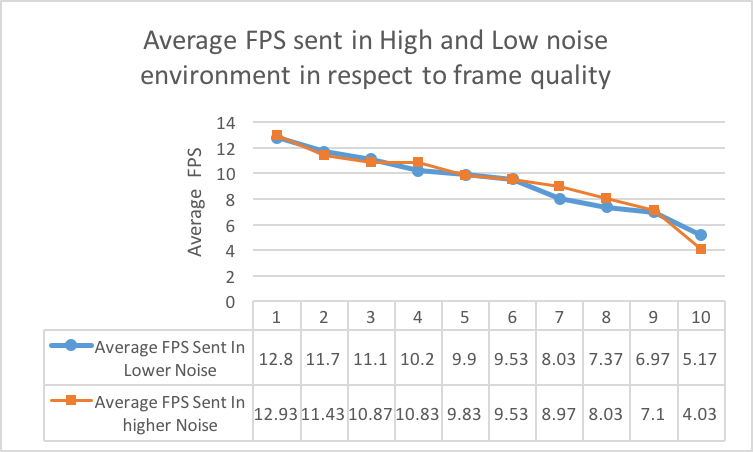
\includegraphics[scale=1]{Figures/Figure17.png}
\caption{FPS in respect to a noisy environment and a quiet environment}
\label{fig:FPSinNoisy}
\end{figure}

To our surprise, the data showed very subtle differences in respect to performance when testing in a noisy environment. In order to make sense of this data, we revisit a section on the frequency-spectrum hopping technique in which BT uses to transfer data. In the Background section, we mentioned that a piece of data, such as our frames, is broken up into tiny little packets spanning approximately 2700 bits long. The lower layers of BT will do this to fit a packet inside 1, 3, or 5 frequency hop time segments. Each second there are 1,600 hop segments, each with 625 microseconds each. With that said, the definition of interference with noise is a random fluctuation in electrical signal in the transmission space that two devices are connected under. That is other devices or natural phenomenons that produce a signal at the same frequencies that the BT devices are transmitting on. However, since BT hops between 79 different channels of 1MHz each, the chances of another interfering device transmitting at the same channel is very low. Thus, we see that noise is really a non-issue when it comes to the performance of BlueStream. 

The last topic we would like to discuss in this paper in terms of environmental factors that may affect the performance of BlueStream may as well be the most obvious one. Nowadays, the processing power of phones vary tremendously based on the price point in which a user buys their phone in. We use the radar graph below to show the difference in performance the two smartphones we used to test our application in which this factor is visualized.

\begin{figure}[h!]
\centering
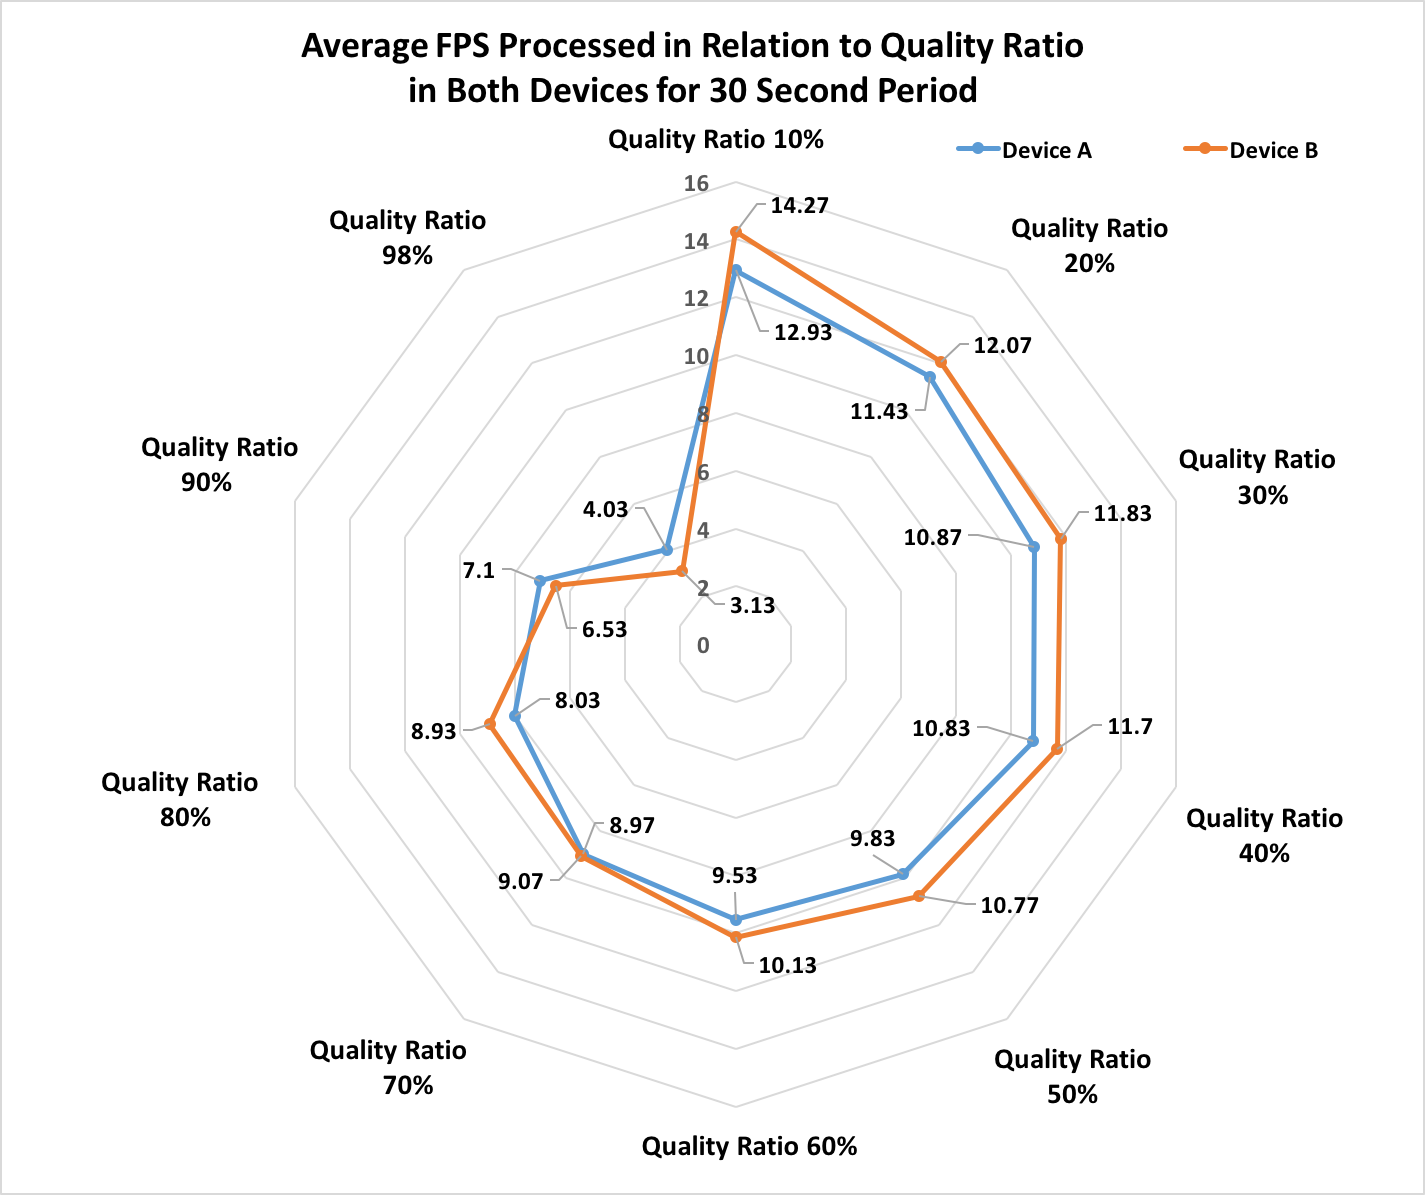
\includegraphics[scale=.6]{Figures/Figure18.png}
\caption{Graph showing the performance of BlueStream on the devices used to test the application}
\label{fig:PerformanceRadar}
\end{figure}

Since hardware plays a large role in the performance of our application, we can derive the performance of our application based on a single bottleneck. Due the broad range of performance among phones, our optimal setting should be considerate in respect to slower phones. Based on the data we collected, selecting a lower frame quality will prove to be supportive on slower phones but will underuse the power of flagship smartphone models. In contrary, selecting a quality level will detriment the usability factor of the BlueStream. We believe, based on Figure \ref{fig:PerformanceRadar}, there exists an intersection of quality to performance at a quality ratio of 60 to 70\%. We observe the least deviation in performance within this bracket. It’s important to note, the devices we tested on are rather on the higher end side of the spectrum of all smartphones which leads us to believe it would be more ideal to lower the quality ratio in support of slower smartphones. We place our assumptions on these findings and looked edged towards real proof by conducting a usability survey on the application to the public. 

\subsection{Usability Survey}

In order to conduct our usability survey, we devised a questionnaire (See Appendix 8) with the primary goal to verify our assumption and data collected from personal experiments. We surveyed friends and strangers throughout Carleton University to find out their personal view on our definitive performance factors distance, quality ratio, device processing time and noise level.

According to the data collected from the survey, most of the respondents chose 3 meter as the first distance metric in which they saw a physical deterioration in the performance of the application. The response to the first question was generally inline with our findings where we observed 4 meters as the threshold before a performance decrease was visible. Up next, we asked the subjects to test the quality ratio which respondents enjoyed using the app under. Most respondents observed that when the quality ratio is 10 where the application received the highest value of FPS, however, a substantial increase in quality was notice as the setting was brought above 60. Sadly after setting quality ratio higher than 60, many said they felt the stream was too choppy and started to lag, hence they believed 60 was just right in terms of performance and quality. Our findings confirmed similar ratios where the optimal settings in both devices seems be within this ratio.

In terms of noise level, we selected various locations such as library, residence commons, the cafeteria, and senior undergraduate laboratory in Hertzberg building to survey our subject because these locations have been measured with our spectrum analyzer tool and found to have the greatest variance in noise level. Unsurprisingly, the result shows that there is not a significant diversity in user experience and performance of our application in any respective survey sites. All the subjects were then asked to use BlueStream for approximately 30 second first on device A, then device B and it was observed the respondents saw a visible difference in the performance of the application. This confirmed our findings that our application is a high resource-consuming application and the slight difference in processing power in such devices can result in a noticeable difference in performance. In addition, when ask about whether bluetooth is a good choice to share screen capture, 90\% of respondents agreed this statement.

Our findings concluded that a quality ratio of 60 is most ideal as it meets the design goals: performance, reliability, and usability. Even though our data indicated a quality ratio of 70 would be more idea over all devices, we agreed as a team that by lower the ratio to 60 will allow less power devices to run our application with ease. 

\subsection{Questionnaire}
\begin{figure}[h!]
\centering
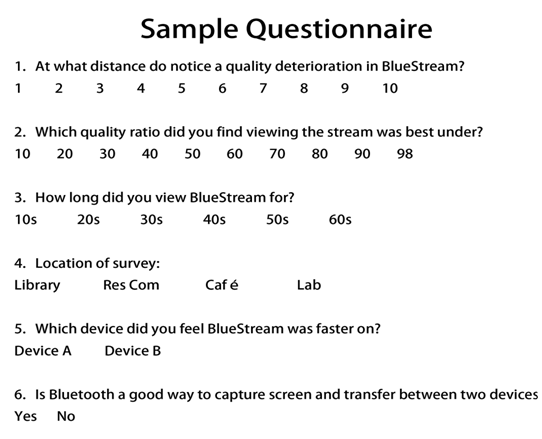
\includegraphics[scale=.7]{Figures/Questionnaire.png}
\end{figure}

\subsection{Result of the Questionnaire}
\begin{figure}[h!]
\centering
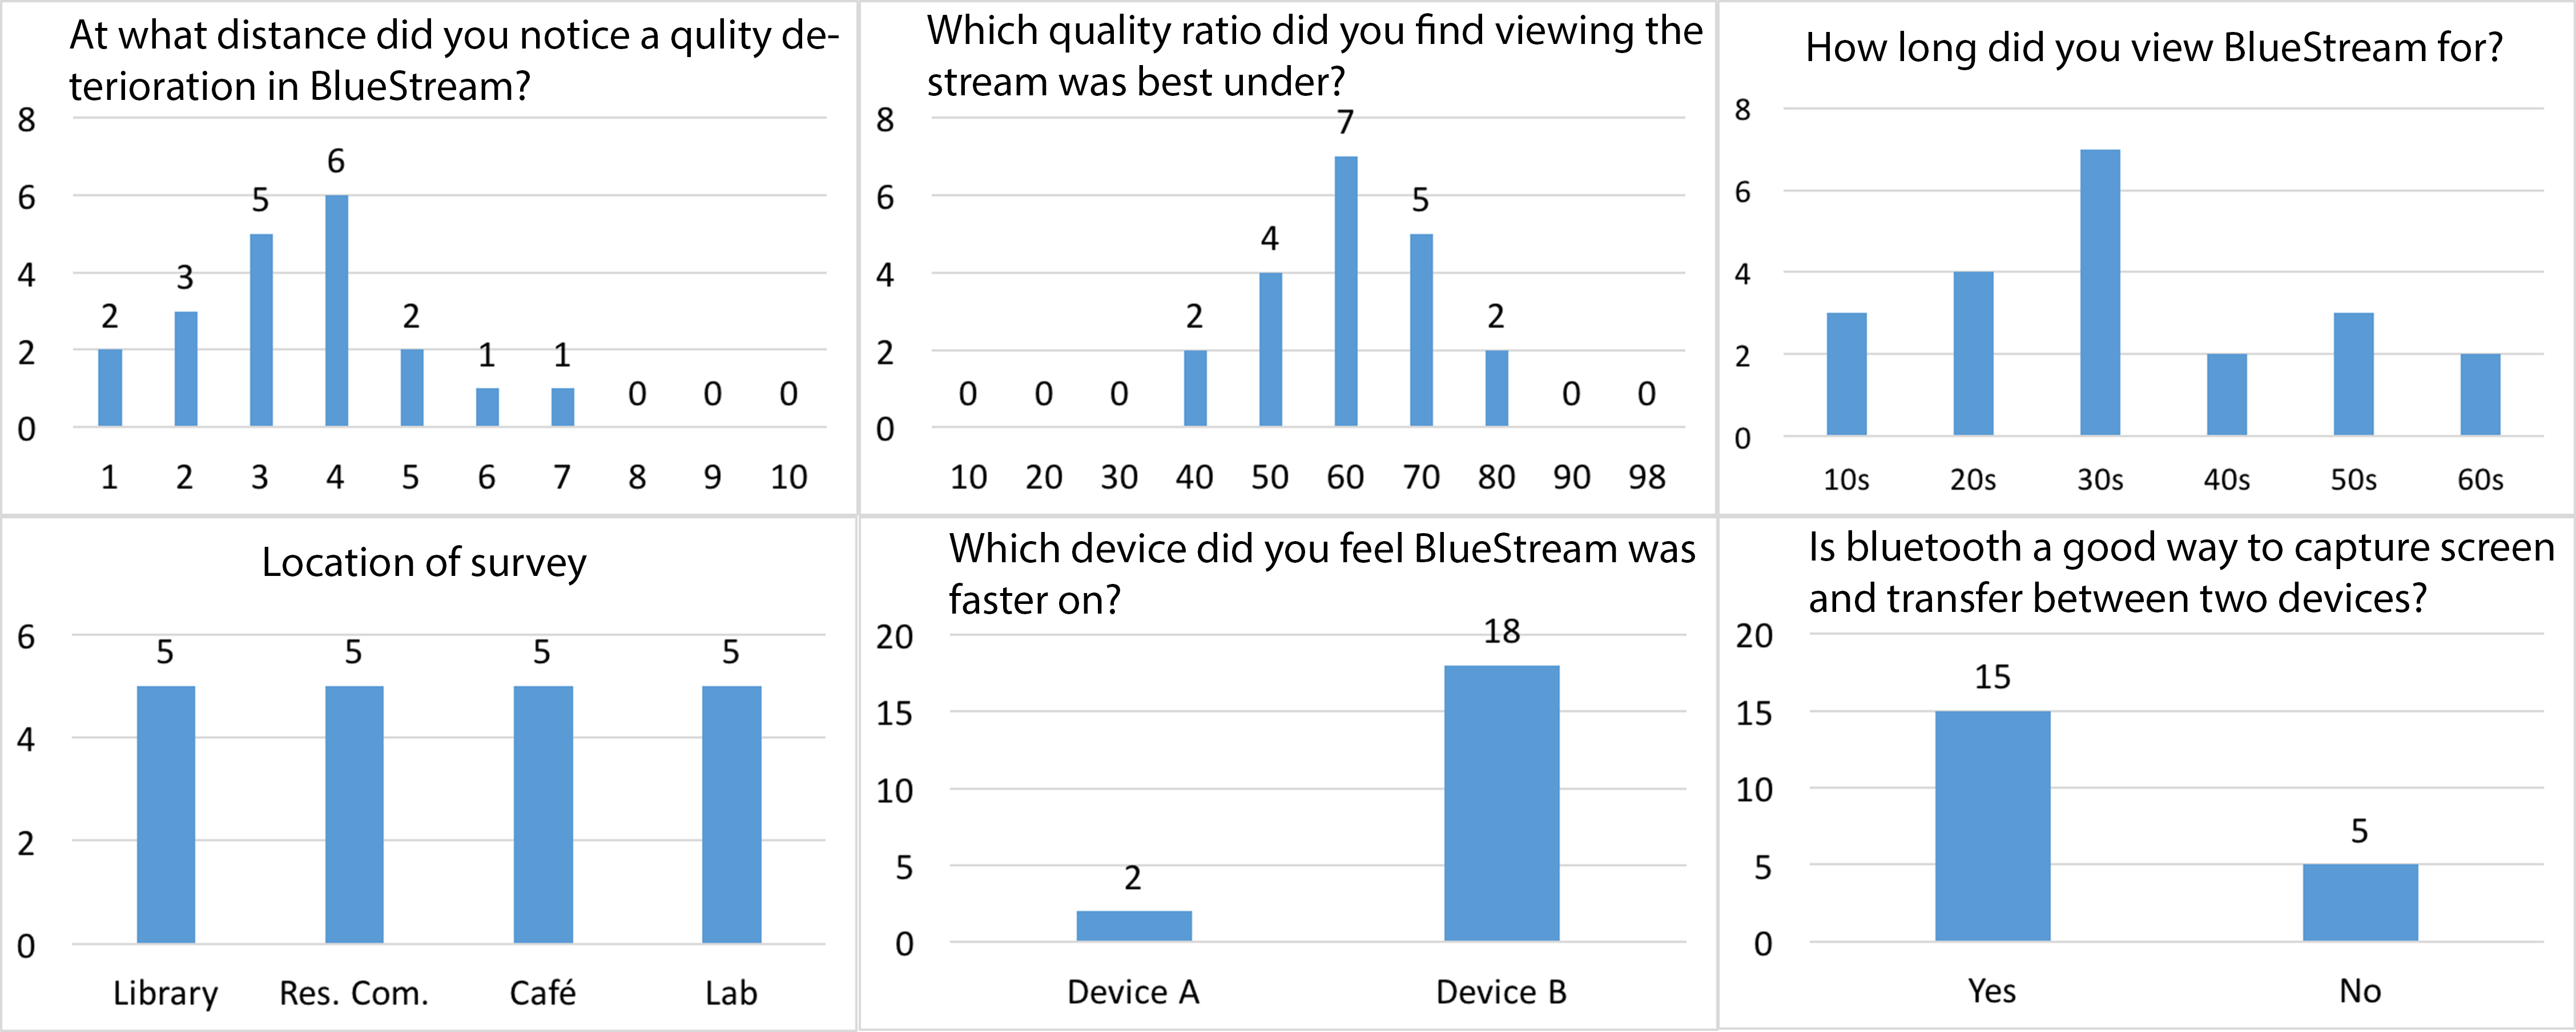
\includegraphics[scale=.4]{Figures/Result.png}
\end{figure}

The graph is demonstrated the best distance will be 4 meter and the best quality is 60\% of every frame. There are a few relation between higher and lower noise. The experience of the questionnaire is spending around 30s and most people believe that Device B is better than Device A and Bluetooth is a good choice to capture screen and transfer the image between two devices.

\section{Conclusion}
Different quality setting leading to a varied size of the image (kB) are the main factors to influence the data transfer rate between two devices running BlueStream. In order to determine the optimal performance setting while maintaining usability of the app, we analyzed the internal and external environment factors that may affect our performance metric: frames per second. The conclusion for an optimal setting in our algorithm was shown through a series of experiments by benchmarking performance of the application under conditions that may expose a slow down accumulated by any internal or external environment factors. We found mixed results in which some of our suspected factors did not influence the performance, and other made all the difference. The distance of the two devices is the single greatest factor that affects the strength of a signal  resulting in a deterioration of the data transfer rate. In addition, we identified the bottleneck of our application to reside on the host device in which the algorithm we designed pays a high computational cost to capture the video stream, frame by frame. Based the data we collected, we came up a hypothesized quality ratio that best served the purpose of BlueStream and sought 20 external participants to verify our findings. According to the experiments and analysis, the observed optimal quality ratio should be set to 60\% corresponding to all the possible environmental and physical factors we considered.

\subsection{Contributions of Team Members}



\begin{thebibliography}{9}
\bibitem{InsideBlueTooth}
Gupta, Naresh, \textit{Inside Bluetooth Low Energy}, Artech House, 2013.

\bibitem{ConnectWithoutCables}
Bray, Jennifer, Charles, Sturman, \textit{Bluetooth: Connect without Cables}, Prentice-Hall, 2001.

\bibitem{BlueToothRevealed}
Miller, Brent, Bisdikian, Chatschik, \textit{Bluetooth Revealed}, Prentice-Hall, 2001.

\bibitem{UnderstandingBTForAndroid}
Pataki, John, “Understanding Bluetooth for Android, iOS, \& Titanium” ,\\\url{logicallabs.com/understanding-bluetooth-for-android-ios-and-titanium/}.\\ Accessed: November 24, 2015.

\bibitem{BTUnifyingTheTelecom}
Bray, Jennifer and Charles, Sturman, “Bluetooth: Unifying the Telecommunications and Computing Industries”,\\ \url{http://www.informit.com/articles/article.aspx?p=27591&seqNum=5}.\\ Accessed: November 24, 2015.

\bibitem{SmartGrids}
Sato, Takuro, \textit{Smart Grid Standards: Specifications, Requirements, and Technologies}, Wiley, 2015.

\bibitem{DevelopersAndroid}
Android, Google, “Developers: Bluetooth Connectivity”. \\
\url{developer.android.com/guide/topics/connectivity/bluetooth.html}.\\ Accessed: November 27, 2015.

\bibitem{MotionJPEG}
Wikipedia, “Motion JPEG”, \url{https://en.wikipedia.org/wiki/Motion_JPEG}.\\ Accessed: November 27, 2015.

\bibitem{SimpleMjpegView}
neuralassembly, “Simple Mjpeg View” , \url{https://bitbucket.org/neuralassembly/simplemjpegview/src}.\\ Accessed: October 27, 2015.

\bibitem{GizMag}
Quick, Darren, “Bluetooth 3.0 goes to 24Mbps via 802.11”, \\\url{http://www.gizmag.com/bluetooth-3-sig/11515/}. \\Accessed: November 29, 2015.

\bibitem{BTSpecs}
Bluetooth, “Basic Rate/Enhanced Data Rate”, \\ \url{bluetooth.com/what-is-bluetooth-technology/bluetooth-technology-basics/br-edr}. \\ Accessed: November 29, 2015.

\bibitem{HPPaper}
Hewlett, Packard, “WiFi and Bluetooth Interference Issues”, \\ \url{http://www.hp.com/rnd/library/pdf/WiFi_Bluetooth_coexistance.pdf}. \\  Accessed: November 29, 2015.

\bibitem{JPEGCompression}
Finell, Damon, Yacoub, Dina, Harmon, Mark, \textit{The JPEG Image Compression Algorithm}, Laboratory of Natural Information Processing, 2015.

\end{thebibliography}

\begin{appendices}
\chapter{Table showing all quality ratio to FPS graph in low performance device when Device A is recording}

\begin{figure}[h!]
\centering
\includegraphics[scale=.95]{Appendix/Appendix1.png}
\end{figure}

\newpage
\chapter{Table showing  all quality ratio to FPS graph in higher performance device when Device B is recording}

\begin{figure}[h!]
\centering
\includegraphics[scale=.95]{Appendix/Appendix2.png}
\end{figure}

\newpage
\chapter{Table showing frames per second in terms of distance (in meters) between connected device when Device A is the record}

\begin{figure}[h!]
\centering
\includegraphics[scale=.95]{Appendix/Appendix3.png}
\end{figure}

\newpage
\chapter{Table showing frames per second in terms of signal for all quality ratio between connected device when Device A is the record}

\begin{figure}[h!]
\centering
\includegraphics[scale=.9]{Appendix/Appendix4.png}
\end{figure}

\newpage
\chapter{Table showing maximum FPS by sending null images}

\begin{figure}[h!]
\centering
\includegraphics[scale=.95]{Appendix/Appendix5.png}
\end{figure}

\newpage
\chapter{Table showing image size (in kilobytes) after compression relations are applied}

\begin{figure}[h!]
\centering
\includegraphics[scale=.75]{Appendix/Appendix6.png}
\end{figure}

\newpage
\chapter{Table showing fps processed in low noise environment }

\begin{figure}[h!]
\centering

\includegraphics[scale=.9]{Appendix/Appendix7.png}
\end{figure}
\end{appendices}

\end{document}